\documentclass[twocolumn]{aastex631}

\graphicspath{{/Users/devaldeliwala/classes/physics129/ECAL_MonteCarlo/images/}}

\usepackage{float} % for 'htp' placement
\usepackage{multirow}
\usepackage{amsmath}
\usepackage{hyperref}
\usepackage{natbib} 
\usepackage{booktabs}
\usepackage{fontawesome} 



\begin{document}

\title{SIMULATING CMS CALORIMETER RESPONSE OF ELECTROMAGNETIC SHOWERS USING
MONTE CARLO METHODS}

\author{Deval Deliwala}
\affiliation{University of California, Berkeley}

\shorttitle{Simulating Calorimeter Response of Electromagnetic Showers}
\shortauthors{Deliwala}

\begin{abstract}
Accurate simulation of electromagnetic shower development within the Compact
Muon Solenoid (CMS) electromagnetic calorimeter (ECAL) is essential for precise
energy measurements in high-energy physics experiments. This study presents a
Monte Carlo simulation that models the longitudinal development of
electromagnetic showers using a one-dimensional approximation. Phase 1 focuses
on simulating the shower profile for 1 GeV incident electrons in a 25 cm long lead
tungstate (PbWO\(_4\)) calorimeter, validating the simulation against
established benchmarks. Phase 2 assesses the detector's linearity and energy
resolution by calibrating the energy deposition and examining its dependence on
varying incident energies (1, 3, 5, and 10 GeV). Phase 3 involves fitting the
energy deposition function to a gamma distribution, extracting parameters that
characterize the shower development. Phase 4 explores the detector's performance
as a function of calorimeter depth, investigating the onset of
non-linearities in energy response and the scaling of energy resolution. The
simulation demonstrates a linear relationship between incident energy and mean
energy deposited, as well as a square root scaling of energy resolution with
energy, consistent with CMS expectations. These foundational phases establish a
framework for further exploration into more complex shower dynamics and detector
performance metrics.
\end{abstract}

\section{INTRODUCTION}
Accurate measurement of particle energies is fundamental to high energy physics
experiments. Electromagnetic calorimeters (ECALs) are essential for detecting
and measuring the energy of electrons and photons produced in particle
collisions (e.g. \cite{PDG2022}). The CMS ECAL, constructed from lead tungstate
(PbWO$_\text{4}$) crystals, is designed to deliver high-resolution energy measurements
crucial for a broad spectrum of physics analyses, including the identification
of Higgs Boson decays and searches for new particles \citep{Brown2007}.

Understanding the longitudinal development of electromagnetic showers within
the ECAL is vital for optimizing its performance and interpreting experimental
data. This study employs a Monte Carlo simulation with simplifying assumptions
to model the longitudinal distribution of charged particles and photons
generated by electromagnetic showers initiated by incident electrons. The work
is divided into four primary phases:

\begin{itemize}
    \item[1.] \textit{Phase 1:} Simulates the one-dimensional longitudinal
        development of an electromagnetic shower for 1 GeV
        incident electrons, validating the simulation against an established
        benchmarks shown in Figure 33.20 of \cite{Groom2019ParticlePassage}. 
    \item[2.] \textit{Phase 2:} Assesses the detector’s linearity and energy
        resolution across multiple incident energies (1, 3, 5, and 10 GeV).
    \item[3.] \textit{Phase 3:} Fits the energy deposition function to a gamma
        distribution, extracting parameters that characterize the shower
        development. 
    \item[4.] \textit{Phase 4:} Examines the detector’s performance as a
        function of calorimeter depth, investigating the onset of
        non-linearities in energy response and analyzing the scaling of energy
        resolution.
\end{itemize}


This paper is structured as follows: Section \ref{sec_2} provides a detailed
description of the CMS electromagnetic calorimeter. Section \ref{sec_3} outlines
the simulation methods, including the assumptions and computational techniques
used in Phases 1 through 4 of the project and presents the
simulation results for each phase. Section \ref{sec_4} offers conclusions and
discusses future work. 


\section{THE ELECTROMAGNETIC CALORIMETER} \label{sec_2}

The CMS electromagnetic calorimeter is a critical component of the CMS detector
at the Large Hadron Collider (LHC). It is designed to measure the energy of
electrons and photons with high precision and is composed of approximately
61,200 lead tungstate (PbWO$_\text{4}$) crystals. These crystals are chosen for their high
density, short radiation length, and fast ``scintillation" properties, which are essential
for the detection of high-energy particles within a compact volume.

Key features of the CMS ECAL include: \citep{CMS2024arXiv2403.15518} 

\begin{itemize}
    \item[1.] \textit{Material Composition}: PbWO$_\text{4}$ crystals serve as the active
        medium, providing a dense material that facilitates the development of
        electromagnetic showers within a relatively short distance.
    \item[2.] \textit{Geometry and Depth}: The ECAL is segmented into a barrel
        region and two endcaps, each consisting of multiple layers of
        crystals. The total depth of the calorimeter is approximately 23 cm,
        corresponding to $\sim$25 radiation lengths, which is sufficient to
        contain the majority of electromagnetic showers initiated by
        high-energy electrons and photons.
    \item[3.] \textit{Readout System}: Each crystal is coupled to a
        photodetector, typically a photodiode or avalanche photodiode (APD),
        which converts the scintillation light into an electrical signal. The
        readout system is designed to handle high rates of particle interactions
        and provide precise energy measurements.
    \item[4.] \textit{Energy Resolution}: The ECAL achieves excellent energy
        resolution, which is critical for distinguishing between different
        particle types and for precise measurements of particle energies. The
        resolution depends on factors such as the number of crystals, the
        quality of the scintillation process, and the precision of the readout
        electronics. 
\end{itemize}

Understanding the longitudinal development of electromagnetic showers within
the ECAL is essential for optimizing its performance and ensuring accurate
energy measurements. This study focuses on simulating this development using a
simplified one-dimensional model, ignoring transverse spreading, laying the
groundwork for more comprehensive
simulations that account for three-dimensional shower characteristics and
additional physical processes.




\section{METHODS} \label{sec_3} 

This section outlines the Monte Carlo simulation approach used to model the
one-dimensional longitudinal development of electromagnetic showers in the CMS
ECAL. 

\subsection{Phase 1: Monte Carlo Simulation of the Charged Particle and Photon
Distribution} 

The objective of Phase 1 is to develop a Monte Carlo simulation that predicts
the longitudinal development of an electromagnetic shower initiated by 1 GeV
electrons in a 25 cm deep lead tungstate (PbWO$_\text{4}$) calorimeter. The simulation aims to
first generate a plot of the average number of charged particles (only
considering positron-electron pairs, as will be discussed shortly) as a function
of the distance from the incident face of the calorimeter. Afterwards the
averaged number
of photons generated via bremsstrahlung is overplotted and compared
against the number of electrons and positrons. The collective results and
distributions for electron, positron, and photon counts are compared
qualitatively to \ref{Groom2019ParticlePassage}, who used an \textit{iron}
calorimeter with an incident energy of 30GeV to assess simulation accuracy. 


\subsubsection{Simplifying Assumptions} 

To make the simulation tractable, several simplifying assumptions are employed.
These assumptions deviate from the real-world behavior of electromagnetic
showers but allow for a foundational understanding of the shower development
process. 

\begin{itemize}
    \item[1.] \textit{Calorimeter Geometry}: The ECAL is modeled as a uniform,
        one-dimensional crystal of PbWO$_\text{4}$  with a depth of 25 cm. Electrons are
        assumed to enter the front face of the crystal with a fixed energy of 1
        GeV and normal incidence.
    \item[2.] \textit{One-Dimensional Shower Development}: Real electromagnetic
        showers develop in three dimensions, exhibiting both longitudinal and
        transverse spread. For simplicity, the simulation employs a
        one-dimensional model, neglecting any transverse spreading of the
        shower. 
    \item[3.] \textit{Discretized Bremsstrahlung}: Electrons lose energy
        primarily through bremsstrahlung. Instead of modeling this as a
        continuous process, the simulation approximates energy loss as discrete
        events occurring at random positions along the electron’s trajectory.
        The probability of a bremsstrahlung event occurring within a
        differential distance $dx$ in the simulation is given by: 
        \[ dP = \frac{dN}{N} = -\frac{dx}{X_0}. \] where $X_0$ is the radiation
        length of PbWO$_\text{4}$ ($\sim$ 0.89cm).  
    \item[4.] \textit{Equal Energy Division}: Upon a bremsstrahlung event, the
        energy is equally divided between the outgoing electron and the emitted
        photon. This is an unrealistic simplification, as the actual
        bremsstrahlung spectrum is peaked at low photon energies.
    \item[5.] \textit{Constant Ionization Energy Loss}: Charged particle's
        ($e^+$ and  $e^-$) lose energy via ionization at a constant rate per
        centimeter penetrated. The energy loss  $dE/dx$ is taken from PDG's
        \textit{Atomic and Nuclear Properties of Materials} online software and
        is $\sim$ 11.5 MeV lost per radiation length  $X_0$. Therefore, 
        \[ \frac{dE}{dx} \approx 12.92 \frac{\text{MeV}}{\text{cm}}. \]  
        The simulation also ignores the Landau distribution of energy loss and
        the Bragg peak effect as particles come to rest. 
    \item[6.] \textit{Photon Interactions}: Photons interact primarily through
        electron-positron pair production in this simulation. The chosen
        probability of pair production within a differential distance $dx$ is
        given by 
        \[ dP = \frac{dx}{\frac{9}{7}X_0}. \]
        Upon pair production, the resulting electron and positron share the
        photon's energy \textit{equally}, and electrons are treated as massless
        particles. 
\end{itemize}

\subsubsection{Simulation Procedure} 

The simulation follows these steps for each event: 

\begin{enumerate}
    \item[1.] \textbf{Initialization}: Start with a single 1 GeV electron at the
          front face (\(x = 0\) cm) of the 25 cm long PbWO\(_4\) calorimeter.
      \item[2.] \textbf{Track Management}: Maintain a list of active particles
          (electrons, positrons, and photons) with their respective energies and
          positions.
      \item[3.] \textbf{Energy Loss and Interactions}:
      \begin{itemize}
          \item[-] For each charged particle, determine the distance to the next
              bremsstrahlung event based on the radiation length \(X_0\).
          \item[-] At each bremsstrahlung event, split the energy equally between the
              outgoing electron and the emitted photon.
          \item[-] For each photon, determine the distance to the possible next pair
              production event using the modified radiation length (\(\frac{9}{7}
              X_0\)).
          \item[-] At each pair production event, generate an electron-positron pair,
              each receiving half of the photon's energy.
      \end{itemize}
  \item[4.] \textbf{Energy Loss via Ionization}: For each charged particle,
          subtract the ionization energy loss per centimeter from its energy as it
          traverses the calorimeter. If a particle's energy drops to zero or
          below, it is removed from the active list.
      \item[5.] \textbf{Position Update}: Advance the position of each particle based
          on the distances traveled during interactions and energy loss.
      \item[6.] \textbf{Event Termination}: Continue the simulation until all
          particles have either exited the calorimeter or been absorbed due to
          ionization energy loss.
  \end{enumerate}

\subsubsection{Data Collection and Analysis} 


Only the number of charged particles ($e^+$ and $e^-$) generated via photon pair
production are considered first. For each simulated event, the positions where
charged particles cross planes at specific depths from the front face of the
calorimeter are recorded. After simulating 1000 events to reduce any statistical
uncertainty, the average number of charged particles crossing each plane is
computed. These averages are then plotted as functions of the calorimeter depth
shown in Figure \ref{fig:1a}. 

 \begin{figure}[htp]
  \centering
    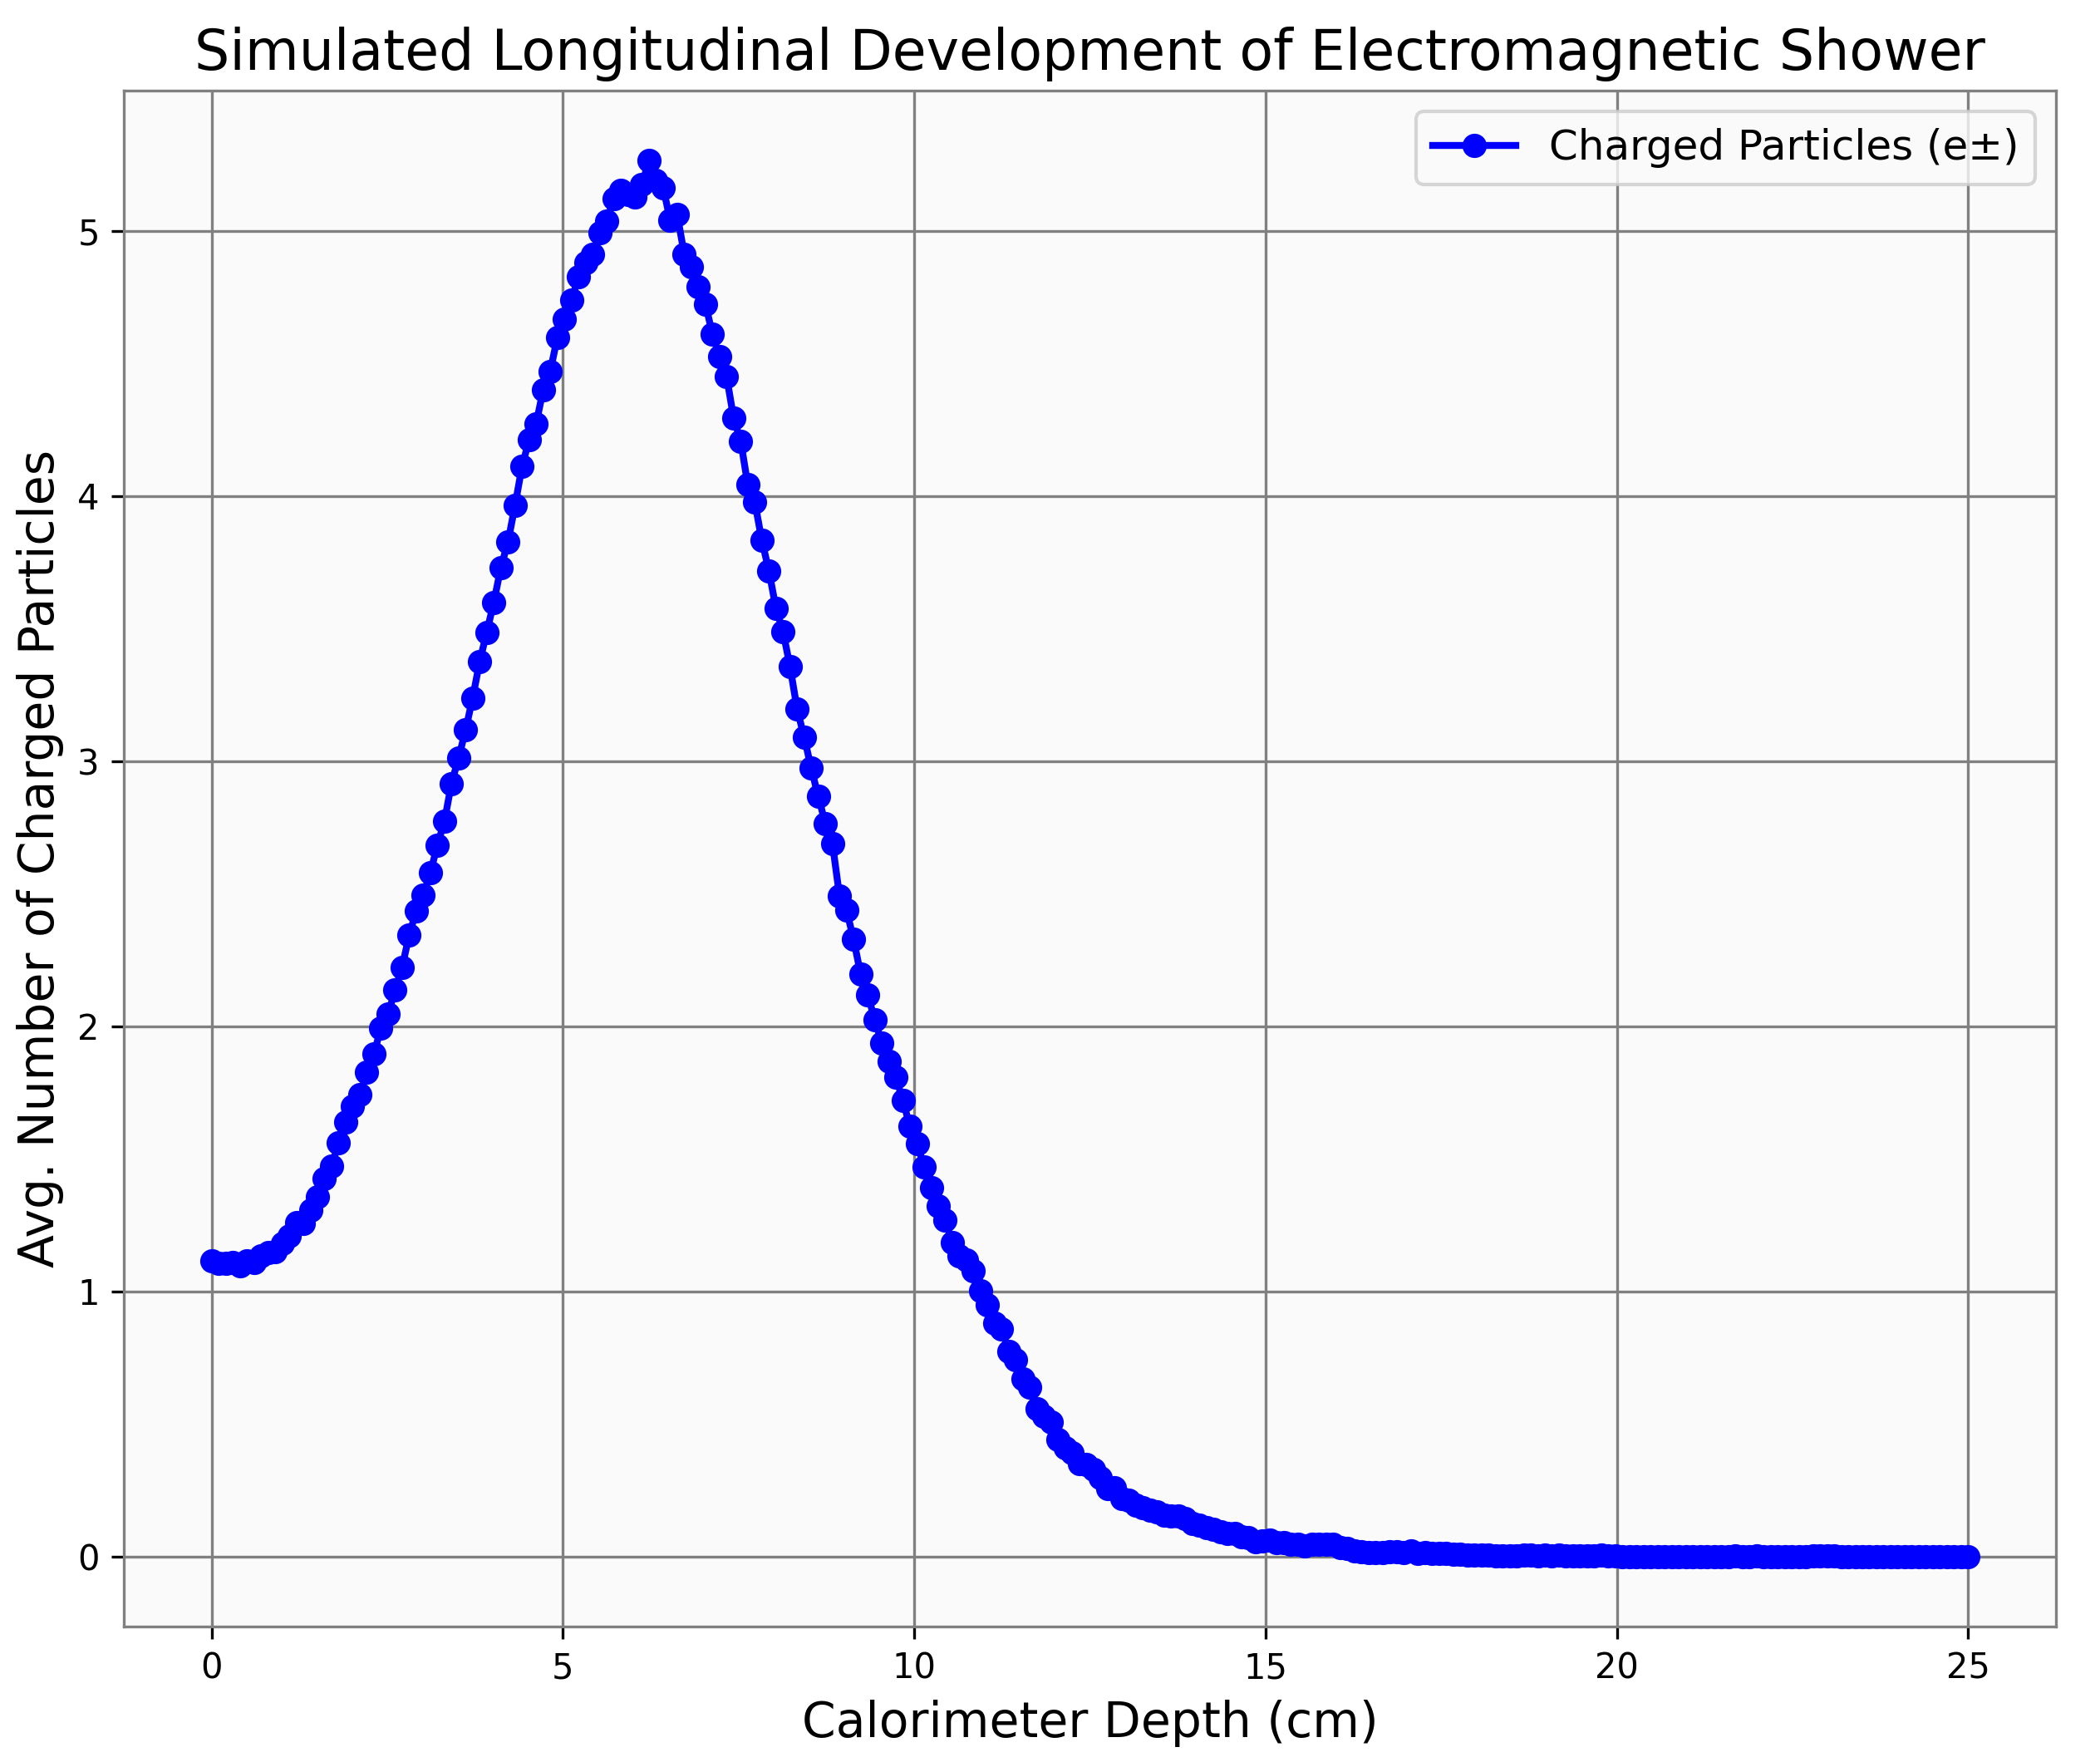
\includegraphics[width = \columnwidth]{part1_a.png}
    \caption{ Average number of charged particles as a function of calorimeter
        depth for 1 GeV incident electrons. The distribution exhibits a peak
        at 6.13cm with $\sim$5 charged particles crossing a plane
        at this depth. The shape closely resembles the charged particle
        distribution shown in Figure 33.20 of \ref{Groom2019ParticlePassage}.}
    \label{fig:1a}
\end{figure}

The above plot shows a similar distribution to the established benchmarks such as Figure 33.20 in
\cite{Groom2019ParticlePassage}, which showcases simulation results 
from an \textit{iron} calorimeter using an EGS4 simulation
\citep{Agostinelli2003} of a 30 GeV electron-induced shower. The number of
charged particles across the calorimeter follows a normal distribution with a
peak of $\sim$95 charged particles at $\sim$6 radiation lengths in iron for a
30 GeV incident shower and a peak of around 5 charged particles at 
$\sim$6.88 radiation lengths in lead tungstate for a 1 GeV incident shower. This
is expected as increased incident energy gives rise to more chances of
pair production occurring which consequently yields more charged particles in the EGS4
simulation relative to the simplified simulation here. 

To ensure the simulated simulation matches the EGS4 simulation PDG performed,
the number of photons across the calorimeter is also considered. As shown in
Figure 33.20 of \cite{Groom2019ParticlePassage}, the photon distribution follows
a similar shape to the charged particle distribution but reaches a lower peak 
\textit{and} at a later depth. More photons afterwards cross larger 
depths of the calorimeter than charged particles. Overplotting the photon
distribution alongside the previously simulated charged particle distribution
showcases similar results to the EGS4 simulation, with photon counts peaking at 
a deeper radiation length and surpassing the number of charged particles
afterwards at increasing depths (see Figure \ref{fig:1b}). Of course, both distributions tend to 0 as the particles
increasingly lose energy and ultimately get absorbed. 

\begin{figure}[htp]
  \centering
    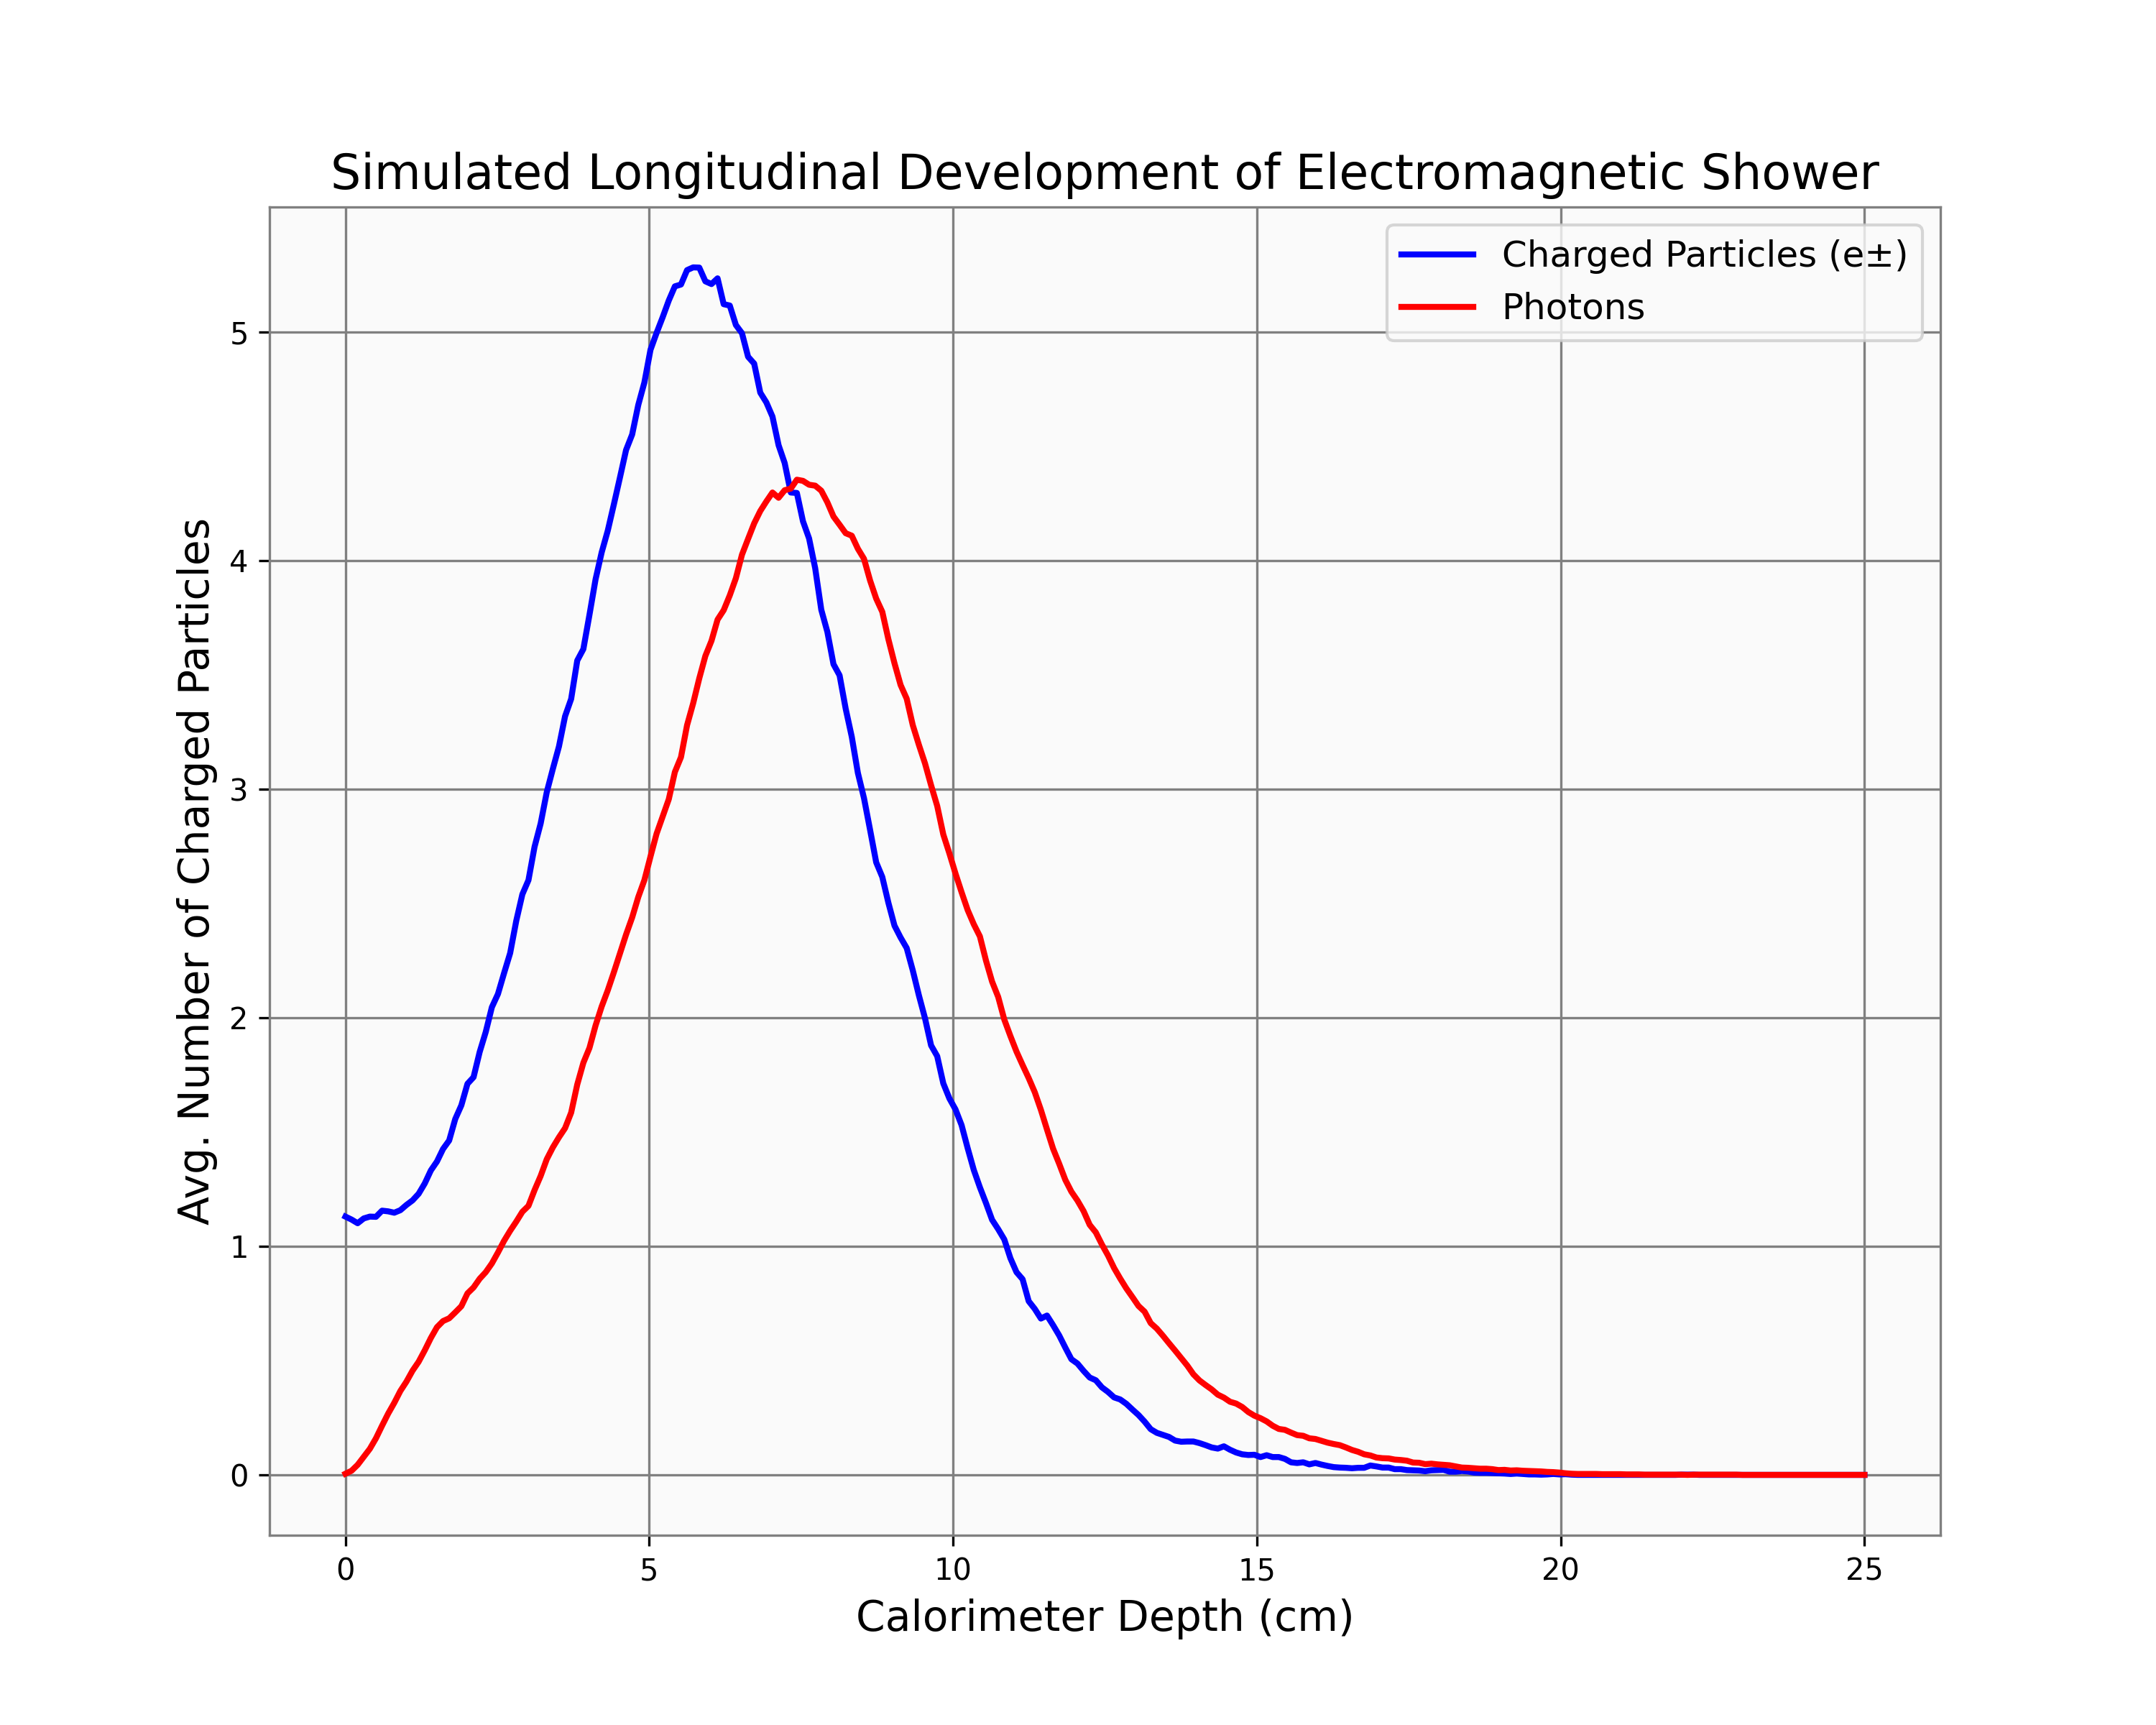
\includegraphics[width = \columnwidth]{part1_b.png}
    \caption{Comparison of average charged particle density and photon density
        as functions of calorimeter depth for 1 GeV incident electrons. The
        number of photons peaks after the charged particles, with the charged particle
        density only surpassing the photon density prior to its peak, in agreement
    with PDG’s EGS4 simulation results \citep{Groom2019ParticlePassage}.}
    \label{fig:1b}
\end{figure}

While the simulation described above employs a one-dimensional model uses a lead
tungstate calorimeter instead of iron,
the general features of the shower development, such as the position of the
shower maximum and the relative densities of charged particles and photons, 
align qualitatively with the PDG benchmarks. Quantitative
differences arise due to the simplifying assumptions and differences in material
properties and incident energies. 

\subsection{Phase 2: Linearity and Energy Resolution of the Detector} 

Phase 2 extends the Monte Carlo simulation to evaluate the detector's linearity
and energy resolution by analyzing the total energy \textit{deposited} in the
calorimeter across varying incident energies. This phase involves calibrating
the simulated detector response and examining the relationship between incident
energy and measured energy deposition. 

\subsubsection{Energy Deposition and Calibration} 

To assess the energy resolution, the simulation tracks the total energy
deposited in the calorimeter from each of the 1000 events. The total energy
deposition is calculated as the integral of the charged particle density along
the entire crystal length, effectively summing the energy lost via ionization.
Photons are excluded from this analysis to focus solely on electron-positron
contributions. 

\paragraph{Initial Calibration} An initial simulation with 1 GeV incident
electrons is used to \textit{calibrate} the detector. When particles of fixed
energy incident energy $E_0$ strike the lead calorimeter, the measured energies from
each particle form a Gaussian distribution in energy centered at $E_0$. The
standard deviation divided by the incident electron energy defines the \textit{energy}
resolution of the detector. Hence, using the initial 1 GeV simulation, the
measured mean of the resultant energy deposition Gaussian distribution is
measured and can afterwards be \textit{scaled} accordingly to yield a
distribution with a mean of 1GeV, thereby calibrating the detector. The measured 
energy resolution normal distribution is shown in Figure \ref{fig:2a}. 

\begin{figure}[htp]
  \centering
    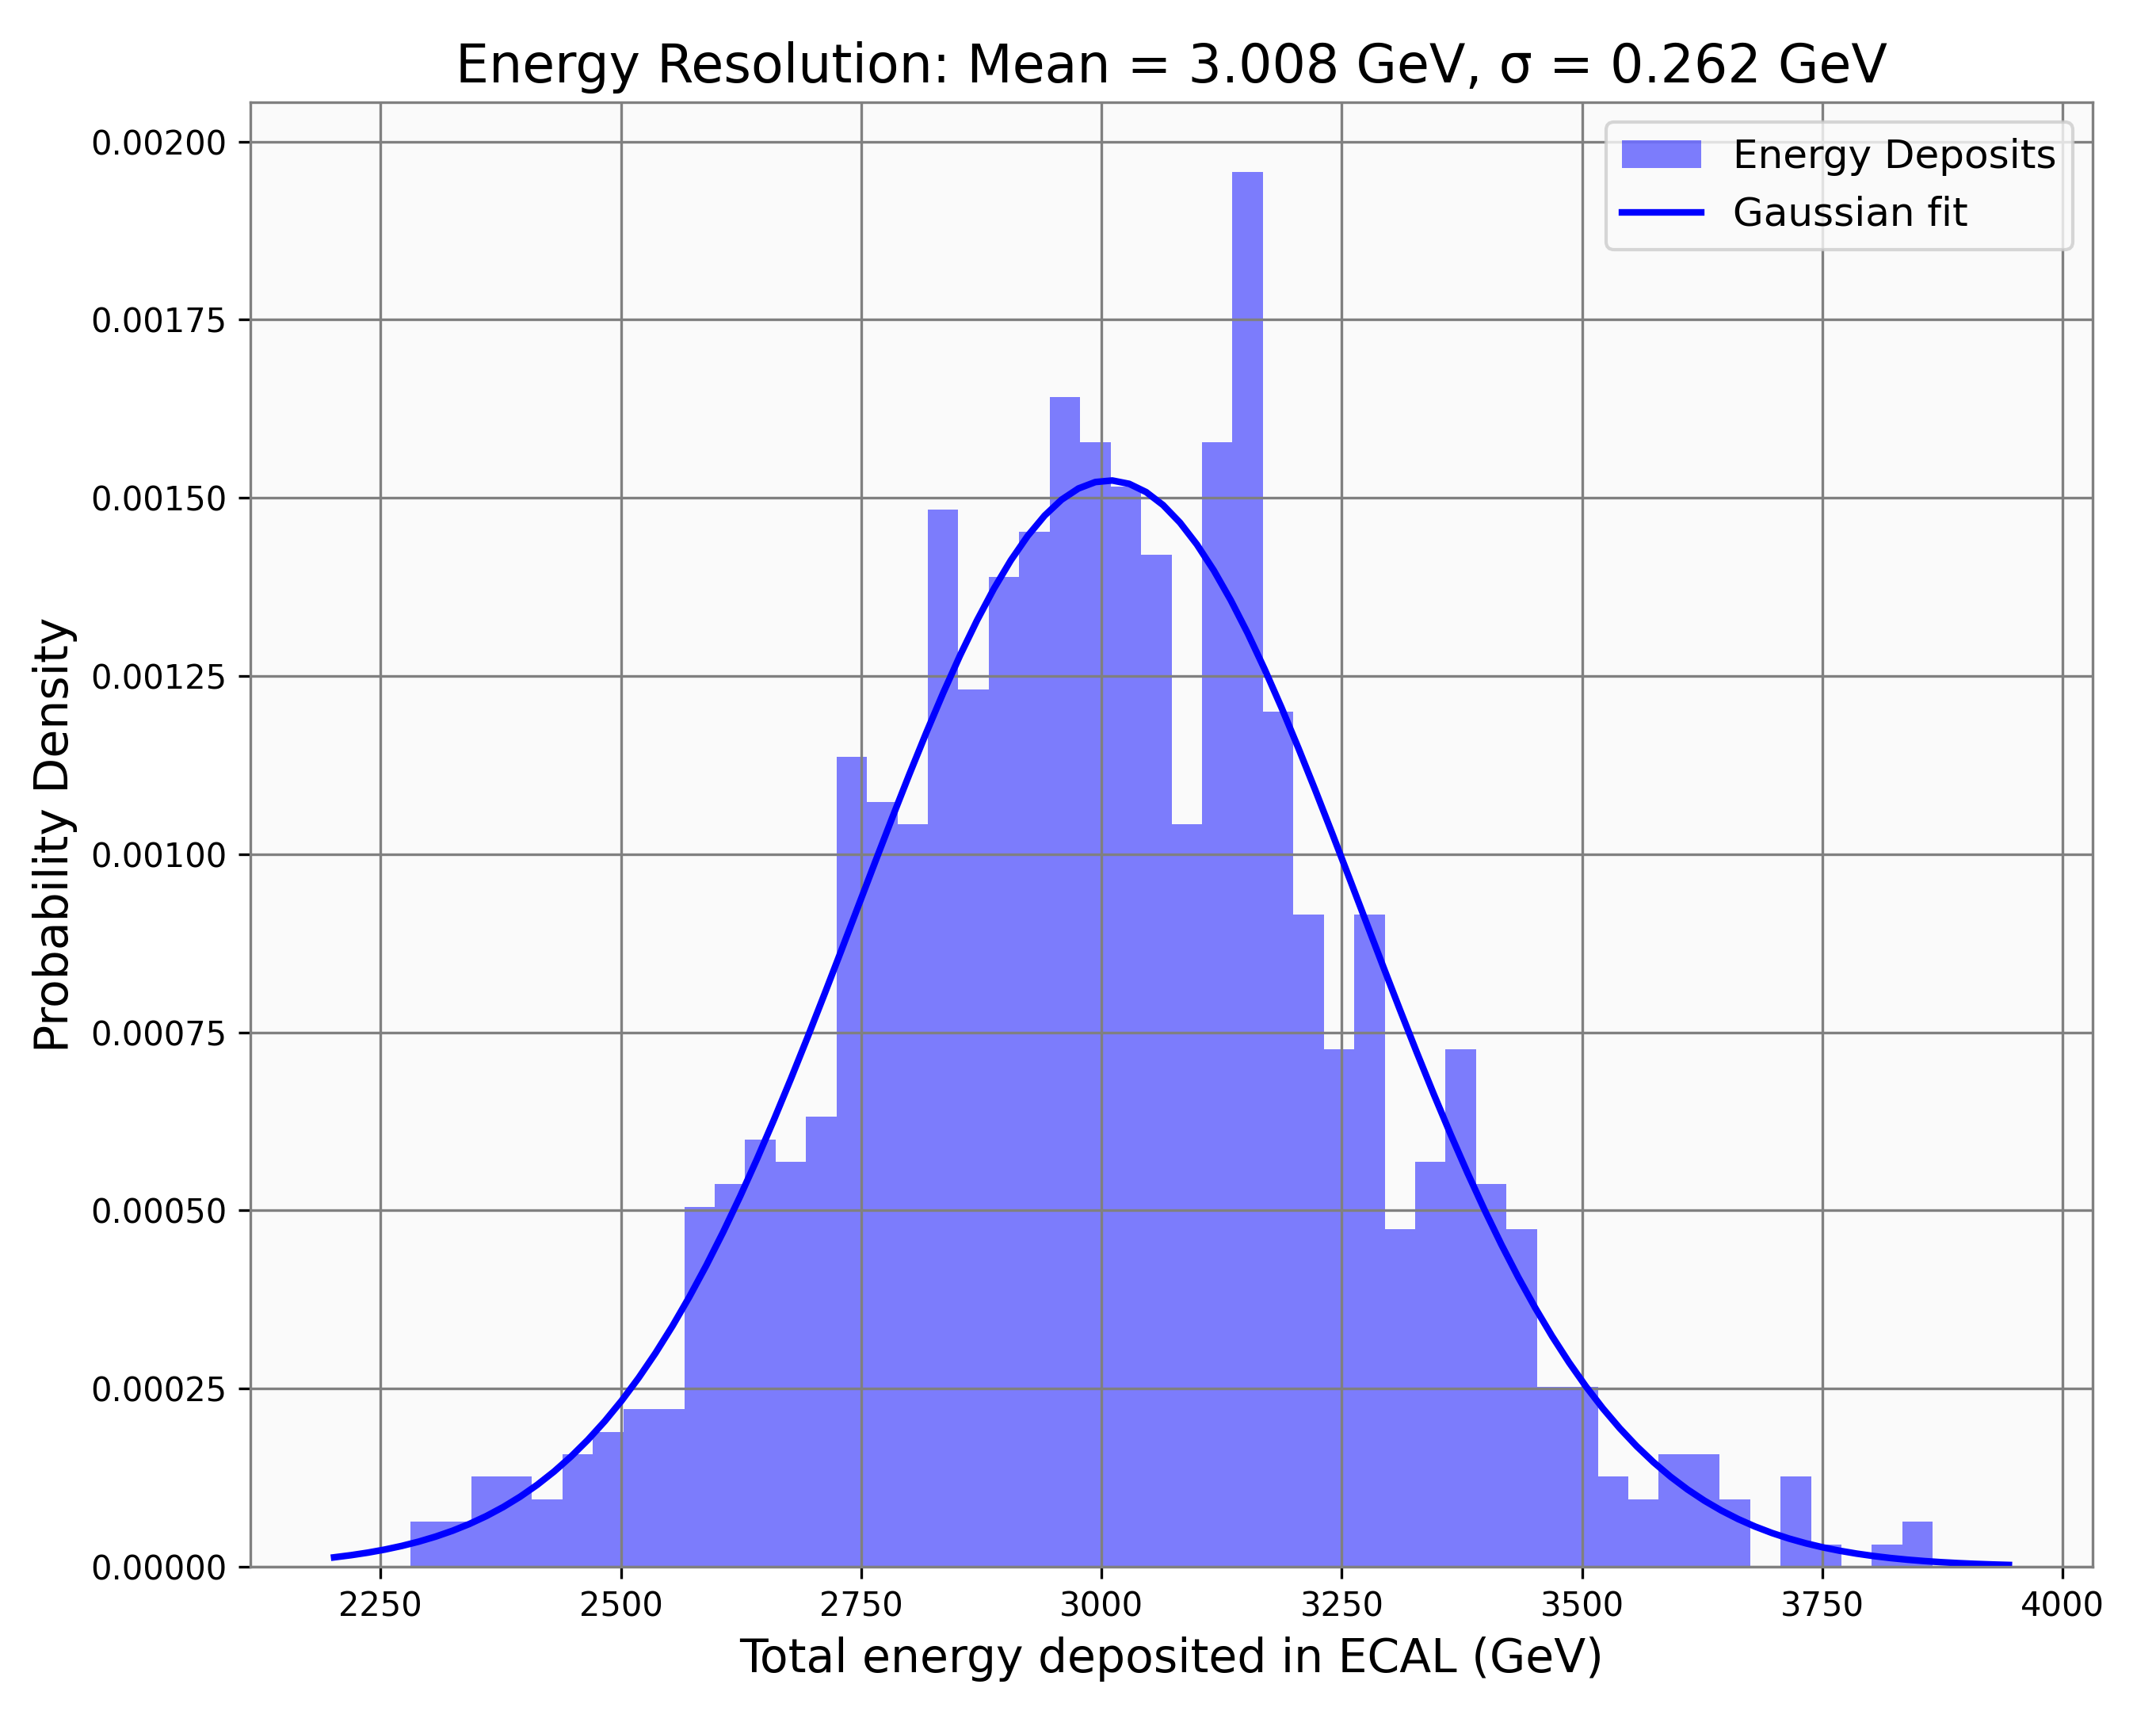
\includegraphics[width = \columnwidth]{part2_a.png}
    \caption{Energy deposition distribution results for a 1000 electrons of 1 GeV
        incident energy. The resultant mean was measured to be 3.008 GeV with a
        standard deviation of 0.262 GeV, hinting the detector should be scaled down by 3x
    for calibration.} 
    \label{fig:2a}
\end{figure}

Therefore, to calibrate the detector, the total energy deposition for each event
was scaled down by 3x, aligning the mean deposition with the known incident
energy. This 3x calibration was consistently effective across multiple incident
energies, yielding histogram means within $\pm 0.03$GeV of the expected values.
The 3x increase in pre-calibrated simulated energy deposits likely stems from
not acknowledging energy conservation and defining ionization loss to be
directly proportional to distance travelled in the calorimeter, without limiting
it to the incident particle's energy. 

\subsubsection{Simulation at Multiple Incident Energies} 

Now that the Monte Carlo simulation is calibrated, it was run for incident
energies of 1, 3, 5, and 10 GeV. For each incident energy, the average charged
particle count as a function of calorimeter depth was measured and is plotted
similarly to Figure \ref{fig:1a} in Figure \ref{fig:2b}. 

\begin{figure}[htp]
  \centering
    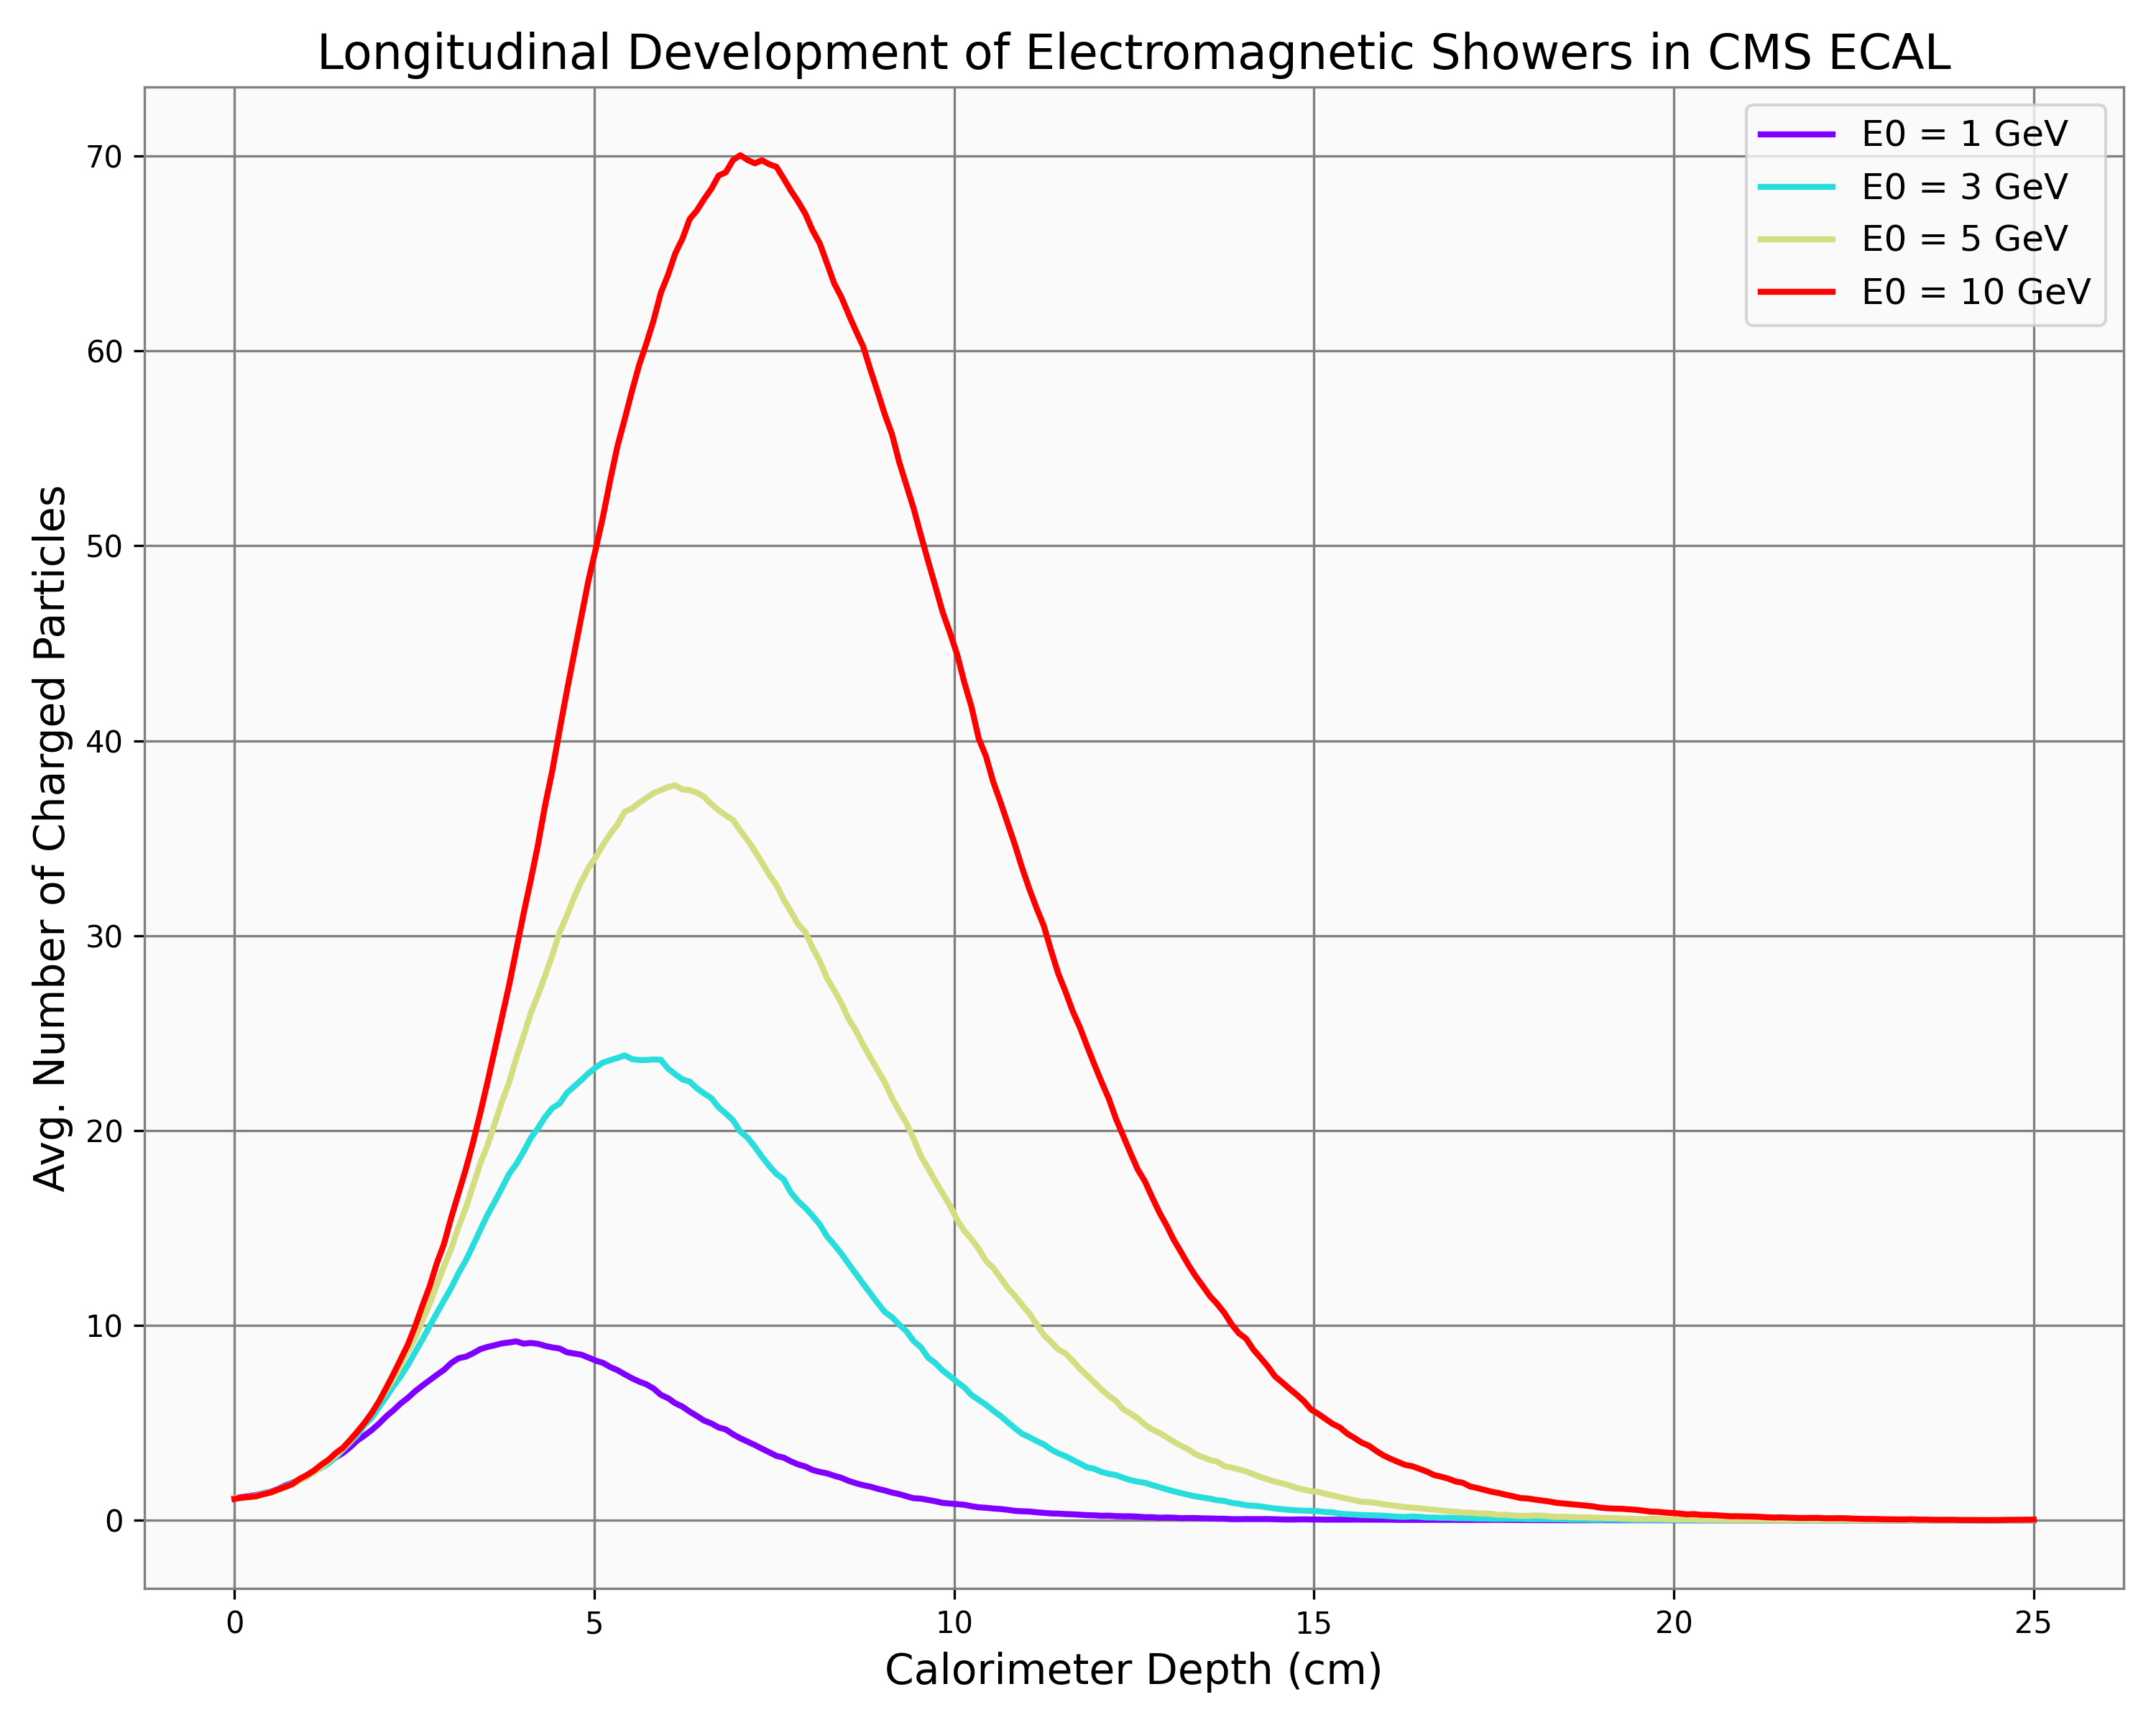
\includegraphics[width = \columnwidth]{part2_b.png}
    \caption{Average number of charged particles as a function of calorimeter
        depth for incident energies of 1, 3, 5, and 10 GeV. Higher incident energies result in
        increased average charged particle densities and further shower
    maximums.}
    \label{fig:2b}
\end{figure}

\paragraph{Results} As the incident energy increases, the average number of
charged particles in the shower increases linearly, while the depth at which
the peak number of charged particles occurs shifts deeper into the
calorimeter. Specifically, the peak occurs 4.01cm at 1 GeV incident energy and
extends to 7.25cm for 10 GeV incident energy, corresponding to 4.5 and 8.15
radiation lengths respectively. The longitudinal distributions maintain a
Gaussian distribution shape, with higher energies resulting in steeper
distributions. 

The relationship between average energy deposited in the calorimeter and the
incident energy was plotted below in Figure \ref{fig:2c}, revealing a perfect linear relationship described
by a slope of 1.00. 


\begin{figure}[htp]
  \centering
    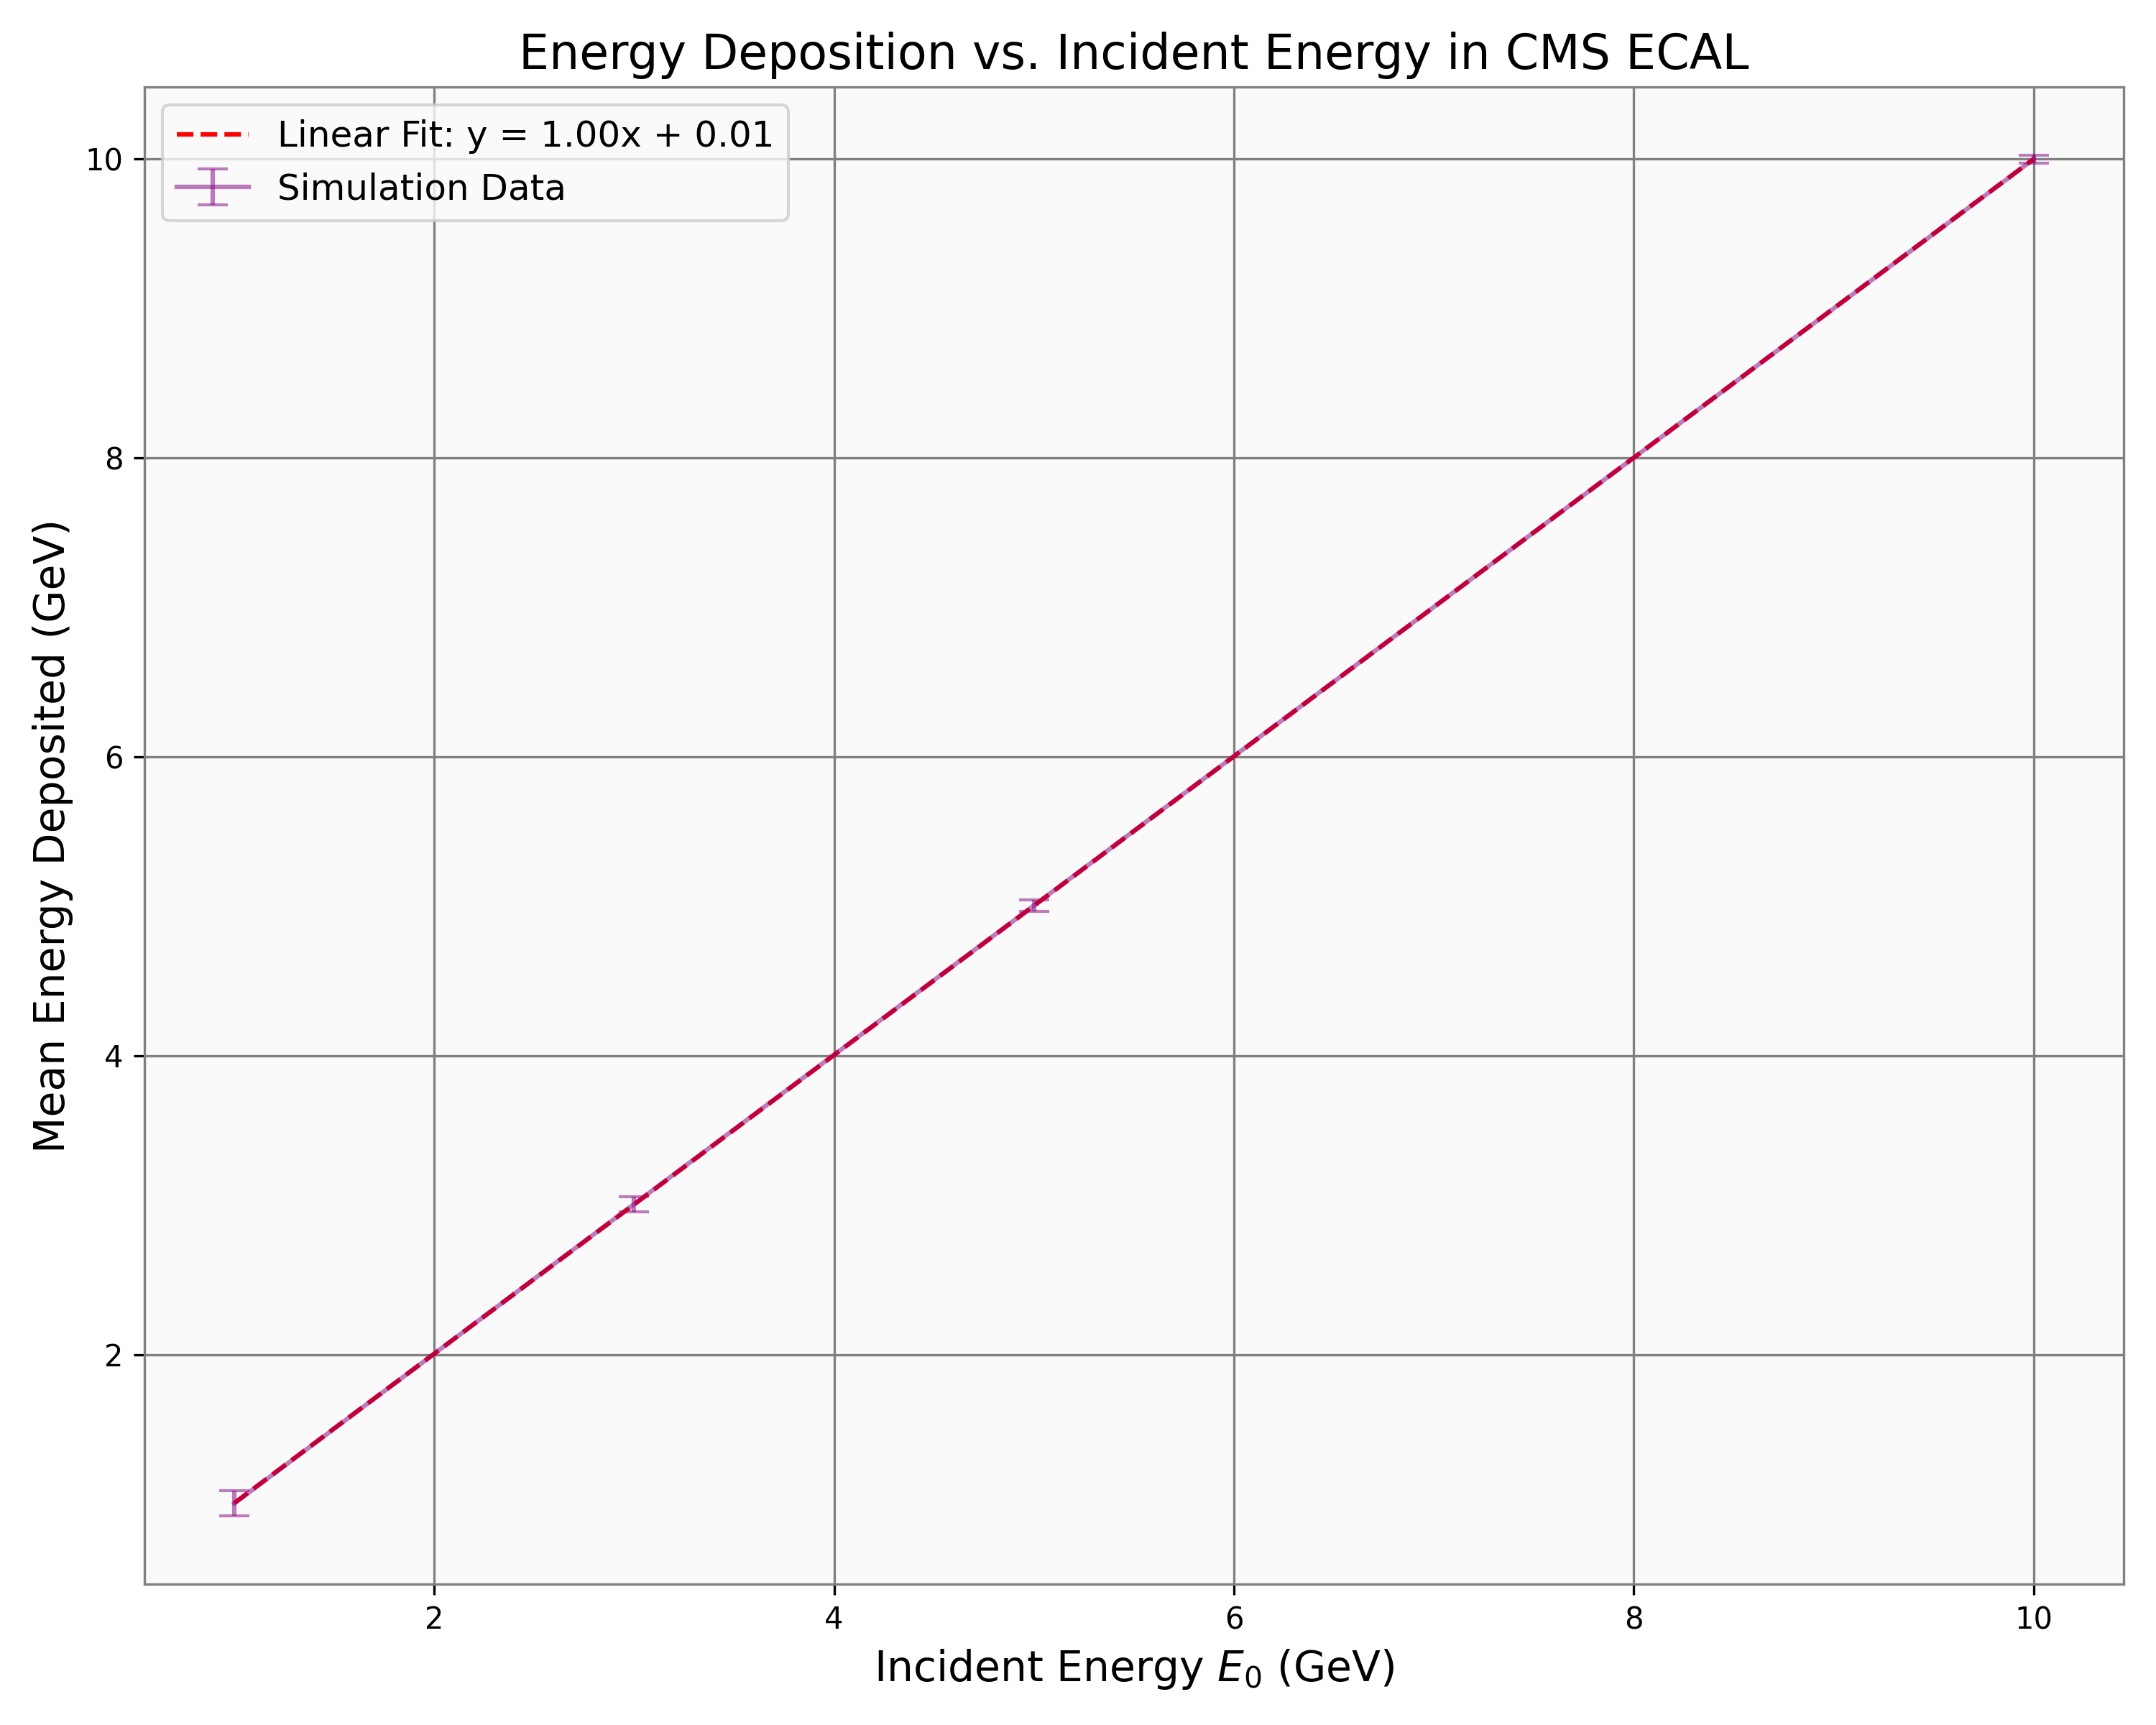
\includegraphics[width = \columnwidth]{part2_c.png}
    \caption{Average energy deposition in the calorimeter as a function of incident
        energy. The relationship is perfectly linear, with a calibration factor
        of 1.00 and an intercept of 0.01, indicating accurate detector
    calibration under simplifying assumptions.}
    \label{fig:2c}
\end{figure}

This linearity is a direct consequence of the simplifying assumptions made in
the simulation, particularly the proportionality of ionization energy loss to
distance traveled and the equal energy sharing in the bremsstrahlung processes.
This relationship is ideal, but not measured in practice due to particle
leakage, radiation, geometrical effects (i.e., particle not entering perfectly
normal), among many other factors that are not considered here. 
 
\subsection{Energy Resolution Scaling} 

The energy resolution of the calorimeter is proportional to the standard
deviation of the total energy deposition of an electromagnetic shower as shown
in Figure \ref{fig:2a} by the equation. To determine how the resolution of the calorimeter
scales with the incident energy, the standard deviation of the energy deposition
distribution divided by the incident energy is plotted against 1, 3, 5, and 10
GeV incident energies like in Phase 1. 

\begin{figure}[htp]
  \centering
    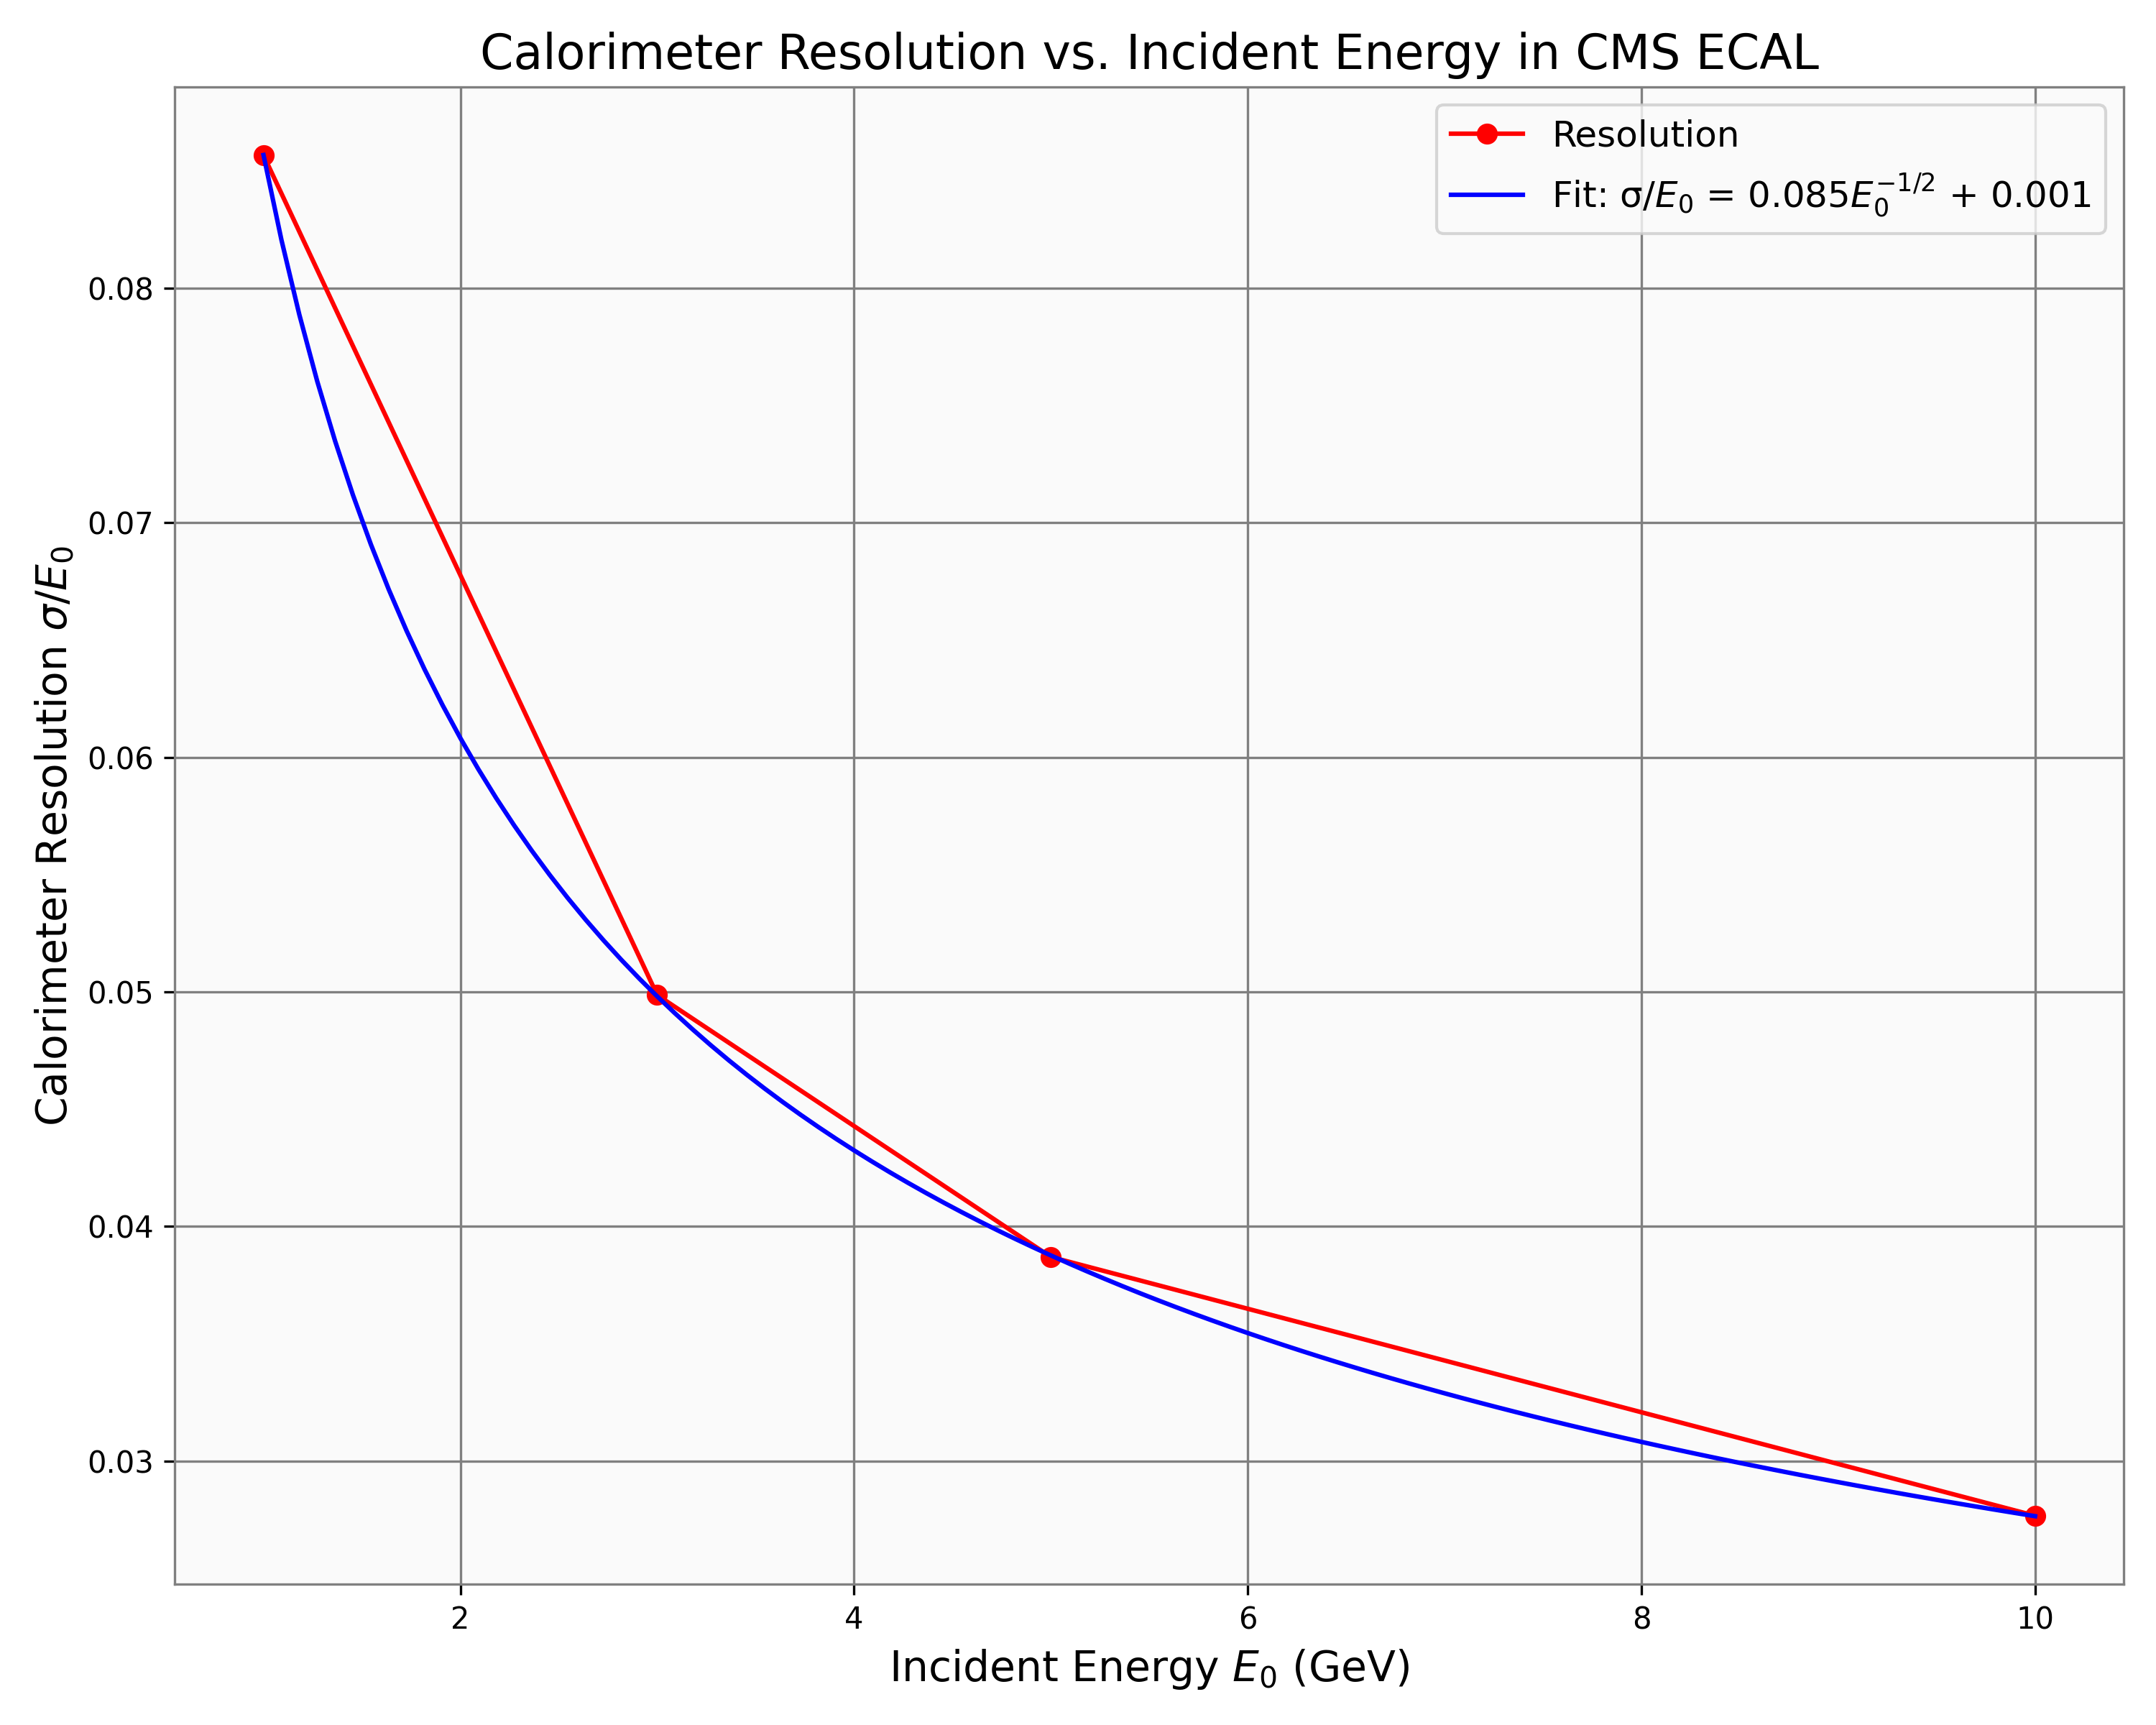
\includegraphics[width = \columnwidth]{part2_d.png}
    \caption{Calorimeter energy resolution ($\sigma/E_0$) as a function of incident energy.
        The resolution follows an inverse square root dependence, fitting the relation
        $\sigma/E_0 = 0.085 1/\sqrt{E_0} + 0.001$, where  $E_0$ is the incident
    energy.}
    \label{fig:2d} 
\end{figure}


The resolution follows an inverse square-root dependence, best described by the fit
$\sigma = 0.085 1/\sqrt{E_0} + 0.001$. This matches the
\textit{inverse} square-root dependence $\sigma / E \propto 1/\sqrt{E}$ that is
typically found in CMS reports \citep{CMS2024arXiv2403.15518}. 

\subsection{Phase 3: Fitting the Energy Deposition Function} 

Phase 3 involves fitting the energy deposition function to a gamma distribution
to characterize the shower development. The energy deposition per unit length is
modeled by the equation 

\[ \frac{dE}{dt} = E_0 b \frac{(bt)^{a-1} e^{-bt}}{\Gamma(a)} \] 

where $t$ is the dimensionless length scale $x/X_0$, with $X_0$ being the
radiation length, and $a,b$ are constants to which the data is fit. Since the
simulation tracks the number of charged particles rather than energy, the
charged particle density is normalized by the total number of charged particles
deposited at 1 GeV, effectively providing a conversion constant from the number
of particles to energy in GeV. 

Using the results from Phase 2, the parameters $a$ and $b$ were derived for
incident energies of 1, 3, 5, and 10 GeV. The results are summarized in Table
\ref{tab:3}.


\begin{table}[htp]
\centering
\begin{tabular}{c||c|c}
$E_0$ (GeV) & $a$    & $b$    \\
\hline
1           & 0.7991 & 0.0030 \\
3           & 0.8622 & 0.0032 \\
5           & 0.8784 & 0.0031 \\
10          & 0.9400 & 0.0037 \\
\end{tabular}
\caption{Energy resolution parameters at different incident energies.}
\label{tab:3}
\end{table}

These parameters indicate how the energy deposition profile evolves with
increasing incident energy, reflecting changes in the shower development
dynamics within the calorimeter. 

\subsection{Phase 4: Linearity and Resolution vs. Calorimeter Depth} 

Phase 4 examines how the performance of the calorimeter changes as a function of
its depth, measured in radiation lengths $X_0$. Specifically, it
investigates the onset of non-linearities in the energy response and analyzes
how energy resolution scales with calorimeter depth.

\subsubsection{Mean Energy Deposition vs. Incident Energy for Varying Depths} 

The simulation was run for calorimeter depths of 5, 10, 15, 20, and 25 $X_0$,
and the mean energy deposition was recorded for incident energies of 1, 3, 5,
and 10 GeV shown in Figure \ref{fig:e_1}. 
 
\begin{figure}[htp]
  \centering
    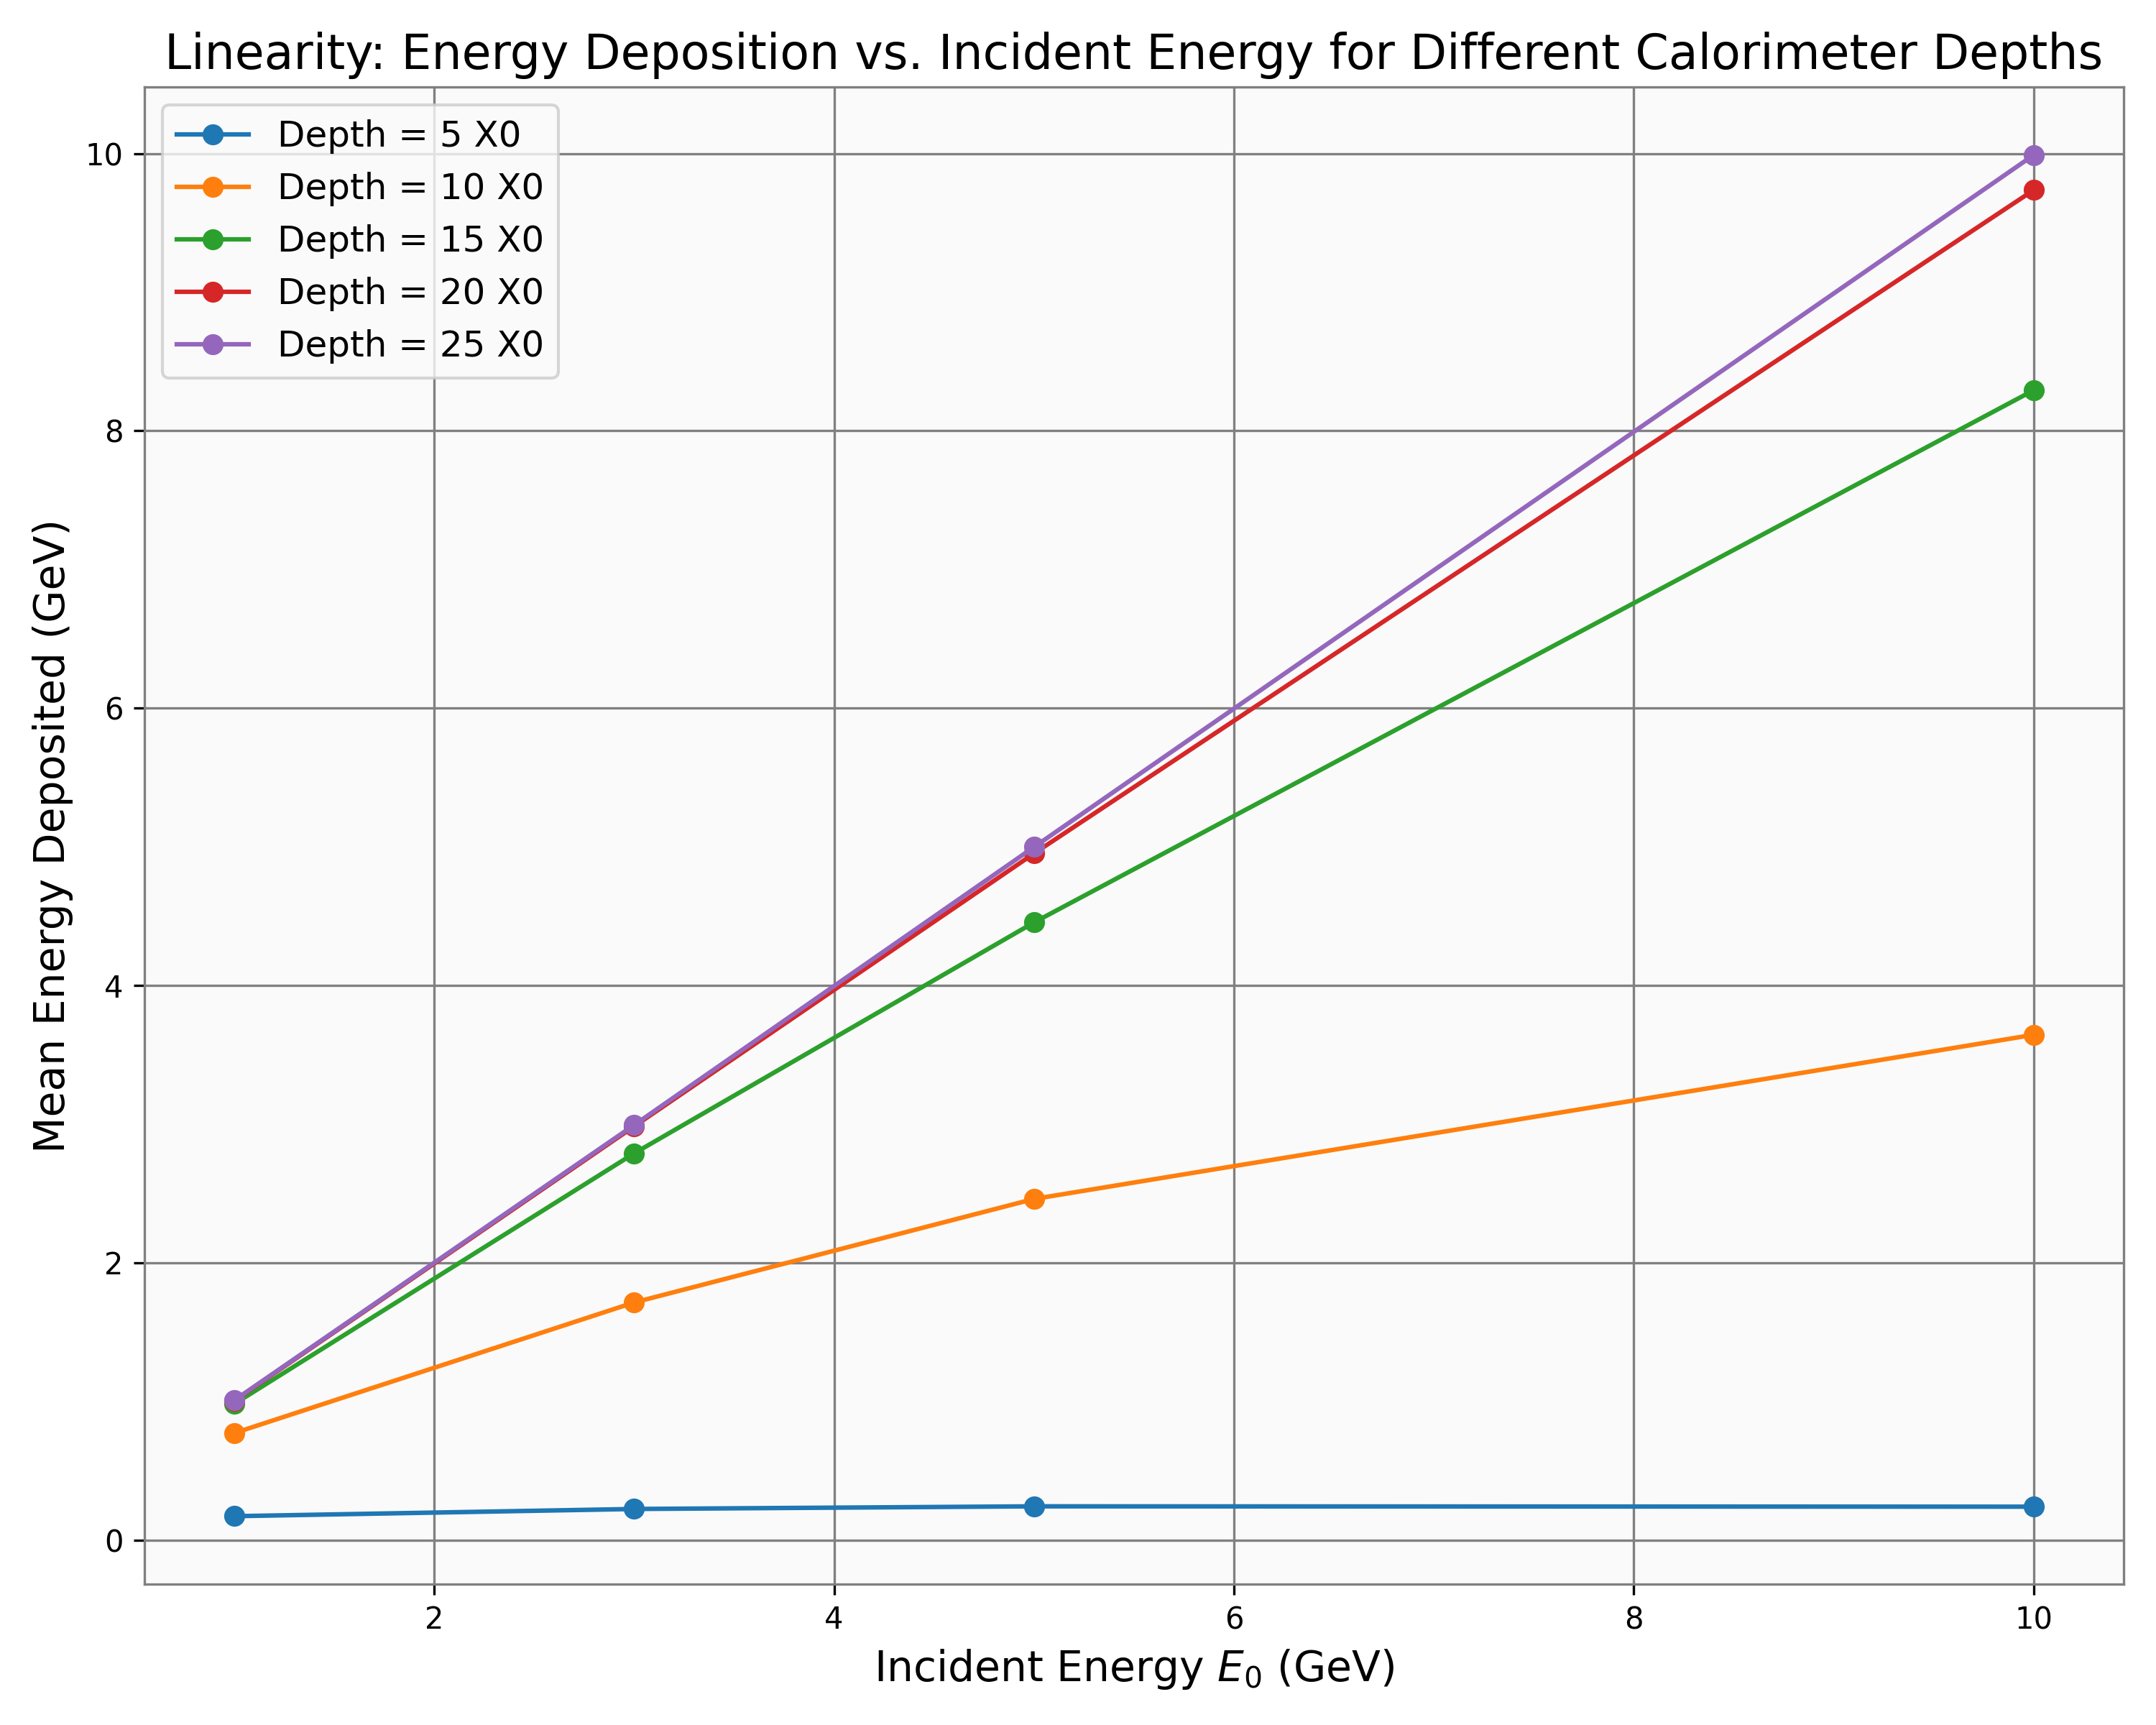
\includegraphics[width = \columnwidth]{linearity_vs_depth.png}
    \caption{Mean Energy Deposition vs. Incident Energy $E_0$ for calorimeter
        depths of 5, 10, 15, 20, and 25 $X_0$ showcasing how energy deposition
    approaches linearity with increasing calorimeter crystal depths.}
    \label{fig:e_1}
\end{figure}


At a calorimeter depth of $5X_0$, the mean energy deposited remained nearly constant,
ranging from depositing 0.26 GeV at $E_0 = 1$ GeV to depositing 0.26 GeV at $E_0
= 10$ GeV. This is expected, as the calorimeter is not deep enough to absorb
the incident particle and its products with the constant ionization energy loss
used in the simulation. Hence the energy deposition is limited by the depth of
the calorimeter, making it equivalent across all $E_0$. Increasing the depth to
10$X_0$, the energy deposition follows a relatively linear trend with a slight
decrease in slope between 5 and 10 GeV. This non-linearity likely
stems from the shower maximum occurring before $10X_0$ at $5$ GeV, but occurring
after  $10X_0$ at 10 GeV. There is a drastic change in the number of particles
capable of being absorbed and depositing energy in the calorimeter between 5 and
10 GeV. Further increasing the crystal depth to 15, 20, and 25$X_0$ resulted in an
increasingly linear trend, with exponentially diminishing differences in energy deposition as
the calorimeter becomes deeper. This is expected as the calorimeter begins to
exceed the maximum depth electrons of incident energy $E_0$ can penetrate, thereby
making the energy deposition at 20$X_0$ nearly identical to $25X_0$.

\subsubsection{Linearity Ratio vs. Incident Energy for Varying Depths} 

The linearity ratio, defined as the mean energy deposition divided by the
incident energy is plotted against the incident energies for various calorimeter
depths in Figure \ref{fig:e_2} 

\begin{figure}[htp]
  \centering
    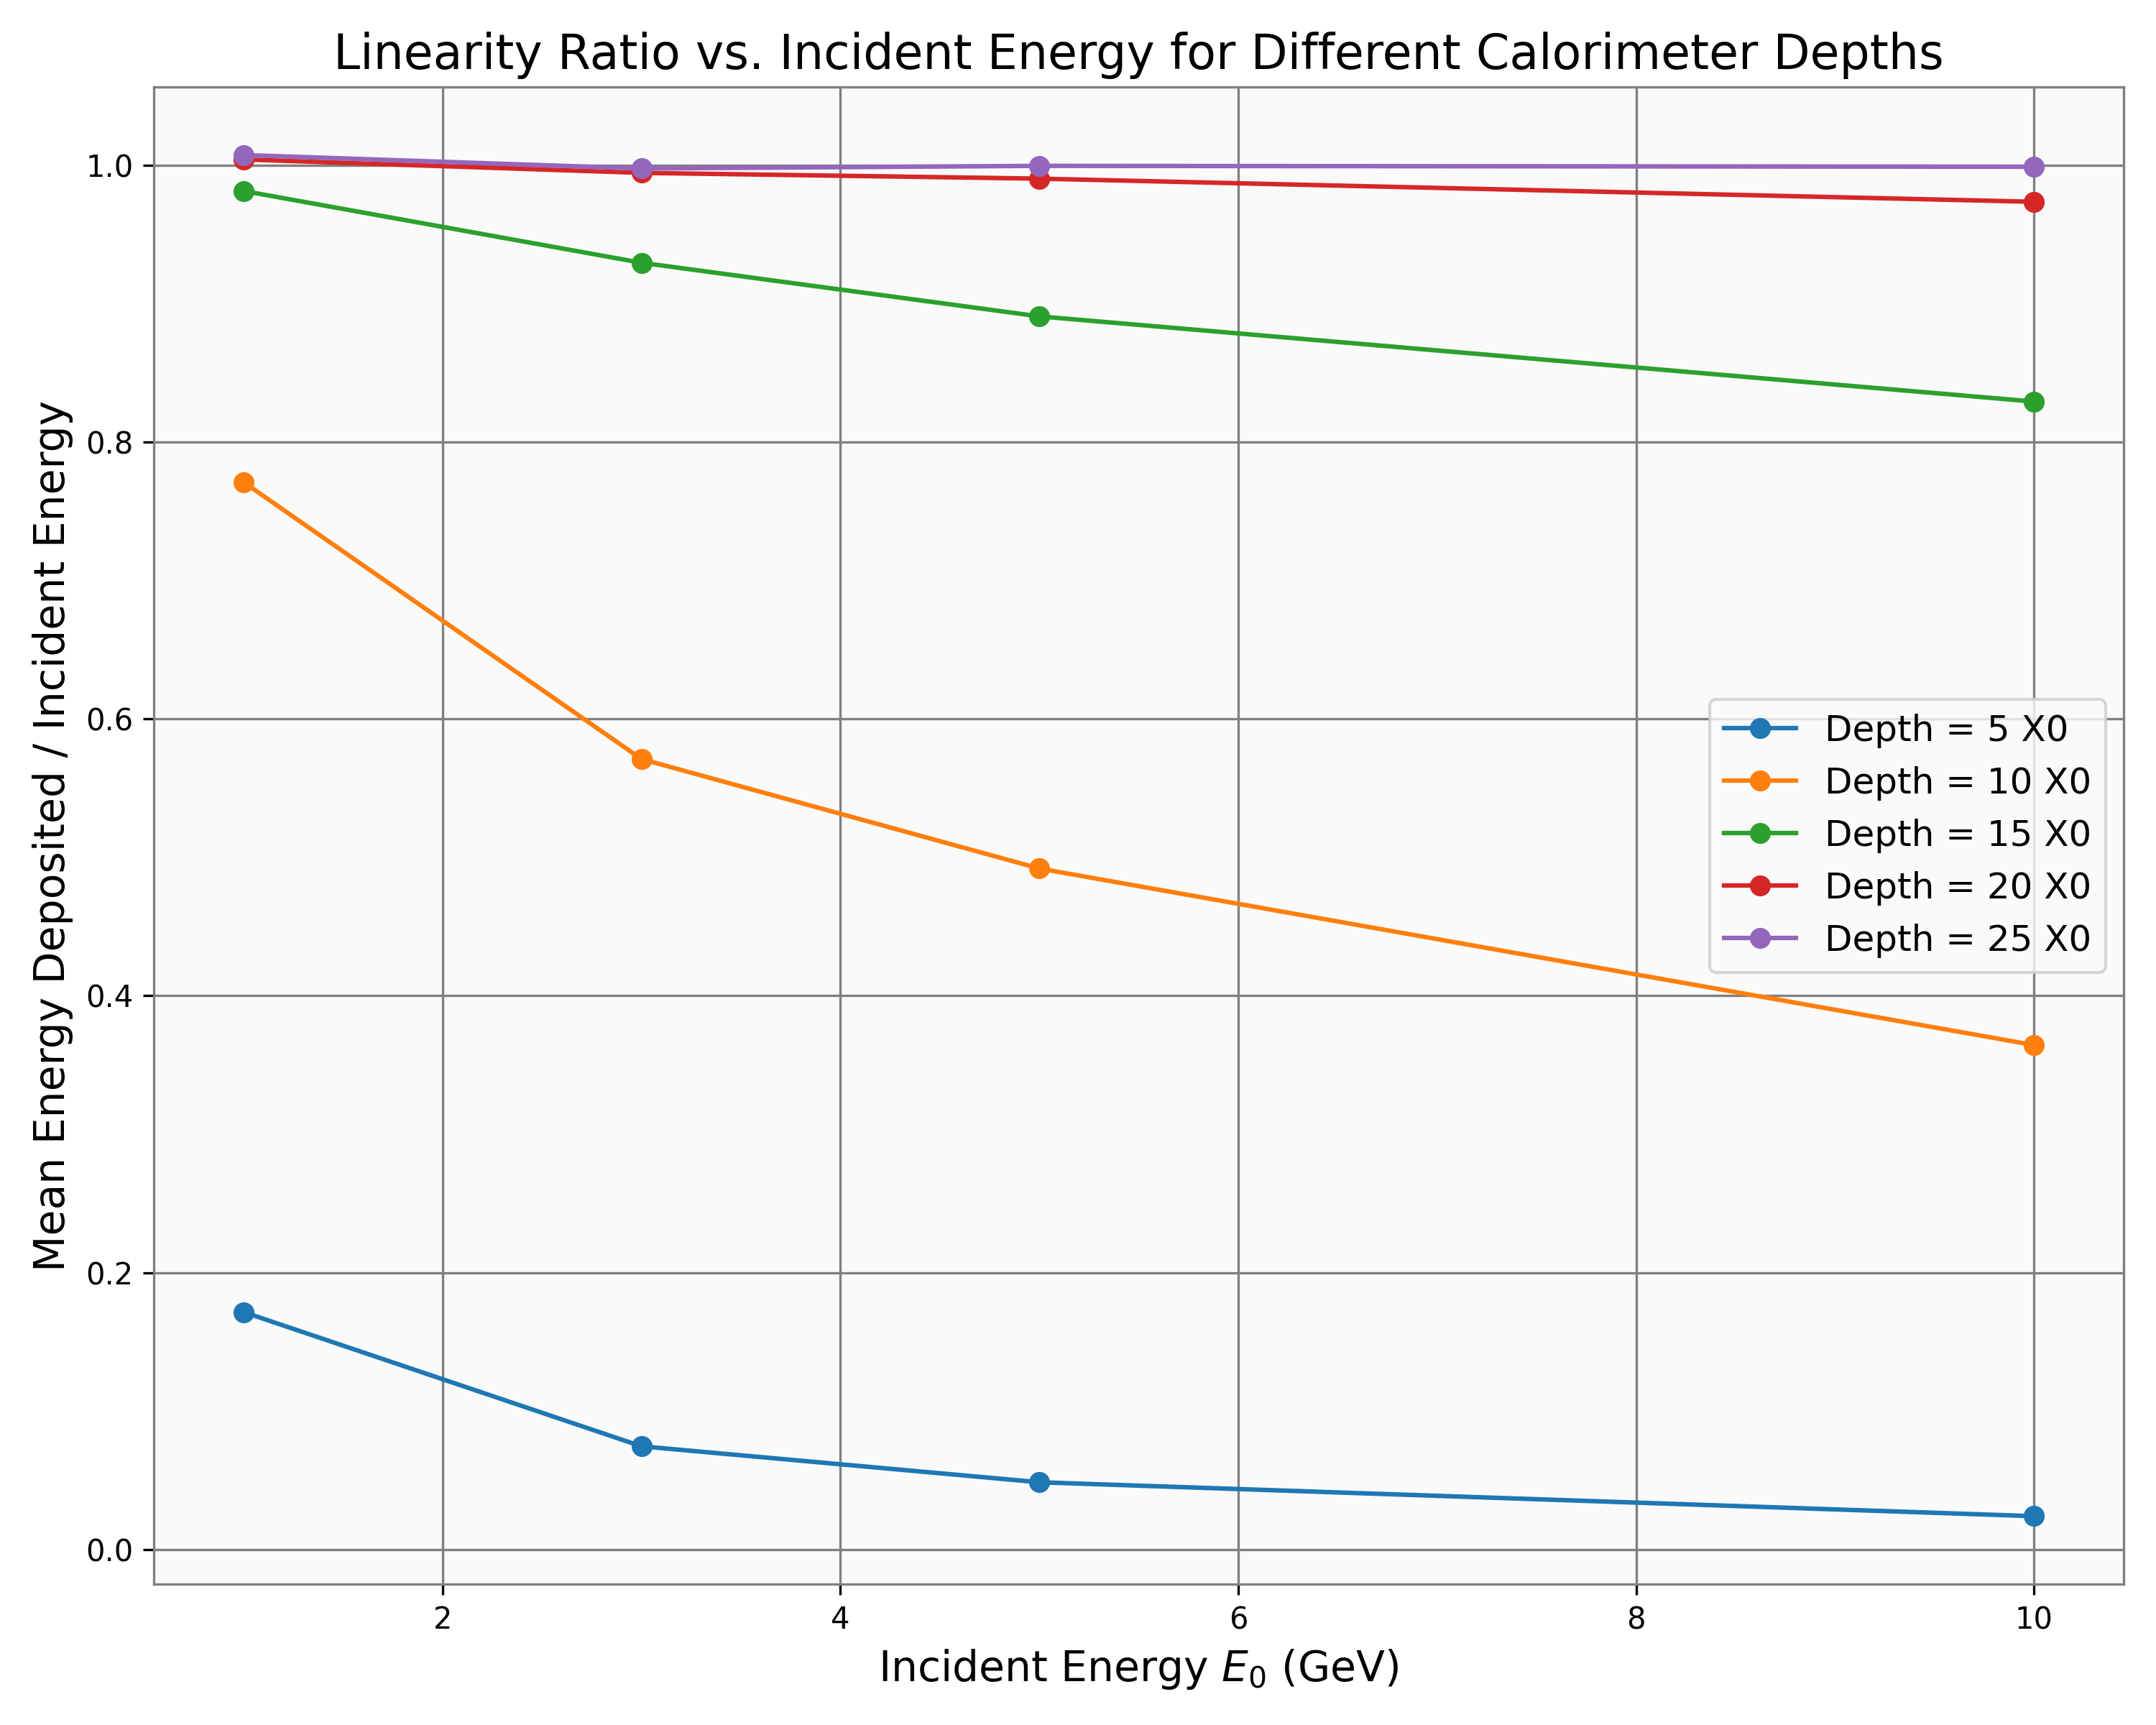
\includegraphics[width = \columnwidth]{linearity_ratio_vs_depth.png}
    \caption{Linearity ratio (Mean Energy Deposited / Incident Energy) vs.
    Incident Energy for different calorimeter depths. Non-linearities emerge at
smaller depths and stabilize at larger depths.}
\label{fig:e_2}
\end{figure}

At a calorimeter depth of 5$X_0$, the linearity  ratio was approximately 0.183 at 1 GeV and
decreased to 0.032 at 10 GeV, following the expected \textit{inverse} square
root trend, flattening with increased incident energy, that was not observed in
Phase 2. At $10X_0$, the ratio was 0.779 at 1 GeV and decreased to 0.383 at 10
GeV, exhibiting a steeper trend. Deeper calorimeters (15, 20, and 25$X_0$) show
reduced differences in linearity across incident energies with trends becoming
more flat as calorimeter depth increases. This overall trend between the
calorimeter depths is expected. At shallower depths like 5$X_0$, electrons
with higher incident energies are capable of depositing progressively smaller fractions of their
initial energies before escaping the calorimeter. At larger depths like $20$ and
 $25X_0$, all of the electron's incident energy is capable of being deposited;
 the electron being ultimately absorbed, resulting in a constant linearity ratio
 of 1.0 across all $E_0$. 

 \subsubsection{Energy Resolution vs. Incident Energy for Varying Depths}

 Figure \ref{fig:e_3} illustrates the energy resolution $\sigma / E_0$ as a function of
 incident energy for calorimeter depths 5, 10, 15, 20, and 25$X_0$. 

 \begin{figure}[htp]
   \centering
     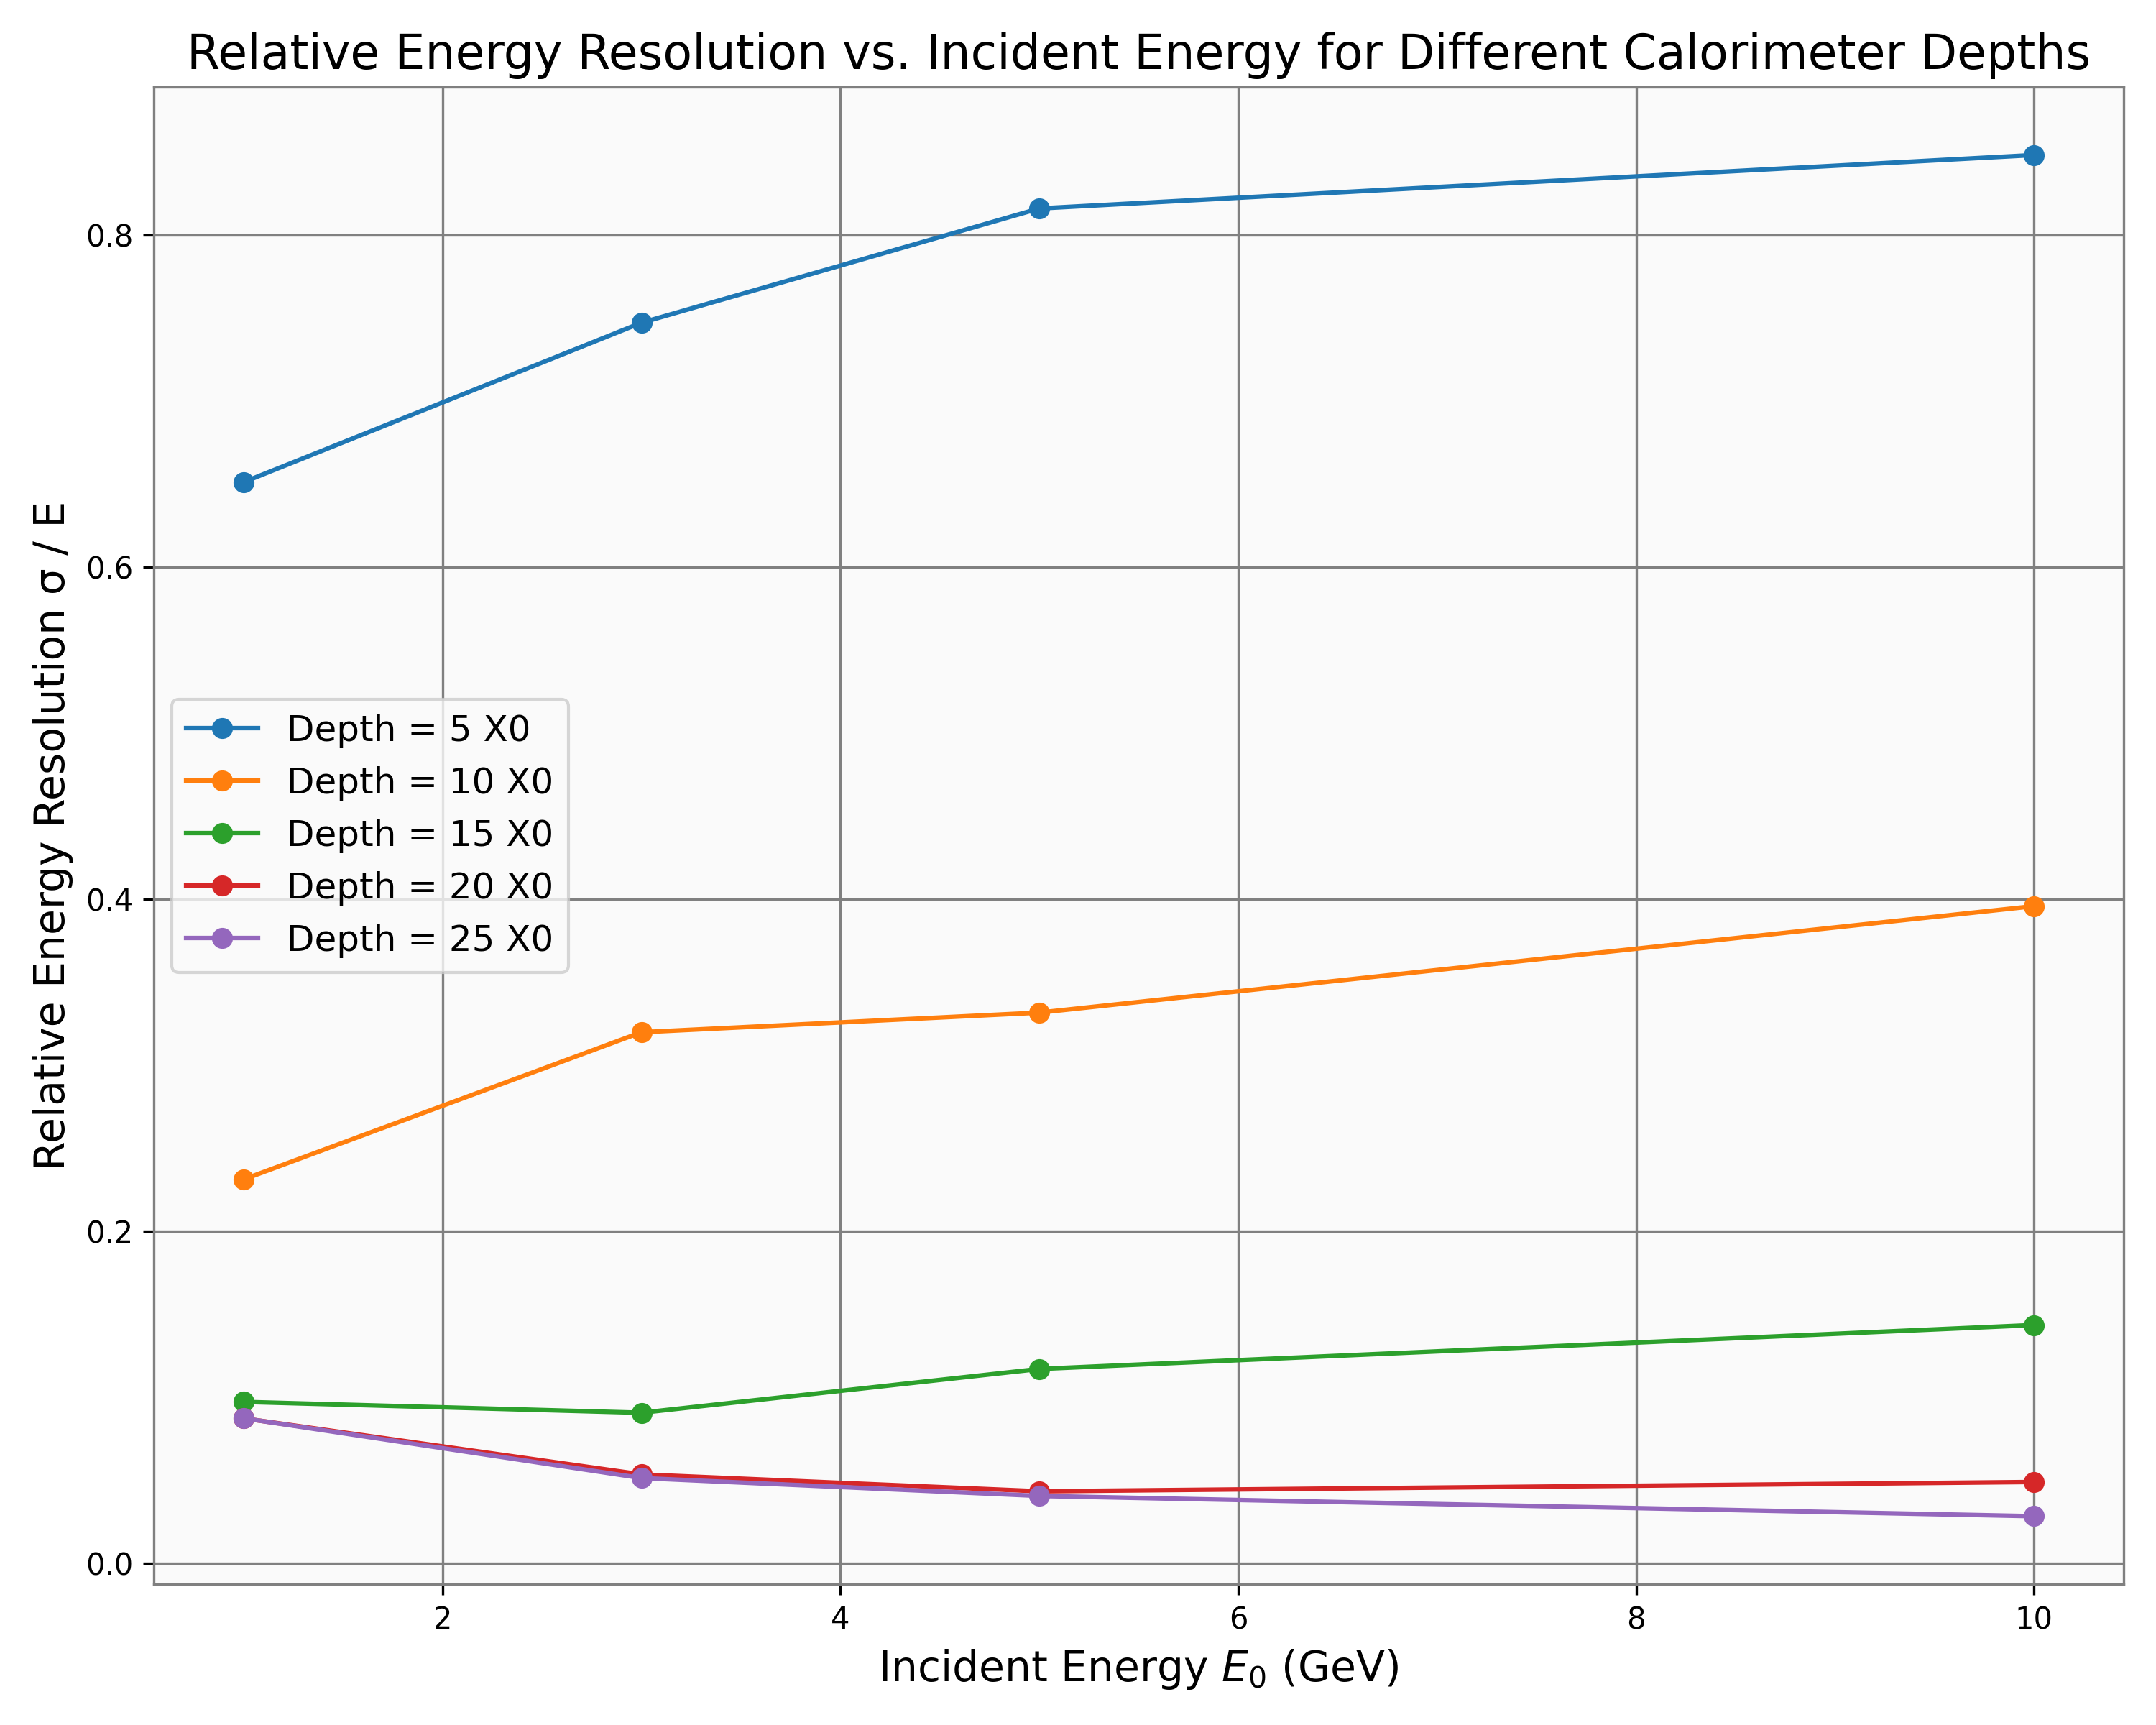
\includegraphics[width = \columnwidth]{relative_resolution_vs_depth.png}
     \caption{Energy Resolution ($\sigma/E_0$) vs. Incident Energy for different
         calorimeter depths. The resolution follows an unexpected square root
         trend for smaller
         calorimeter depths, and follows the appropriate inverse-square root trend for
     larger depths.}
         \label{fig:e_3} 
 \end{figure}



At a calorimeter depth of $5X_0$, the energy resolution was highest, following
an unexpected square-root trend caused by the calorimeter not absorbing all the
energy of the incident electron(s). At a depth of $10X_0$ the resolution becomes less of a
square-root and starts ``becoming" the proper inverse square-root function that
is expected of calorimeter resolutions. At a depth of 20 and 25$X_0$, with the
calorimeters being able to fully absorb the incident electron(s), the resolution
follows the appropriate inverse square-root relationship observed in the CMS
ECAL calorimeter \citep{CMS2024arXiv2403.15518}. Therefore, it seems as
calorimeter depths increase, the energy resolution of the detector becomes
increasingly ``more inverse square-root"-like. Hence, for appropriate physical
detectors that are used in real high-energy physics, a calorimeter of large
depth, sufficient to fully absorb incident particle(s) should be used to maximize
detector energy resolution and readout. 


\section{CONCLUSION} \label{sec_4}
 

This study presents a Monte Carlo simulation of the one-dimensional longitudinal development of
electromagnetic showers in the CMS electromagnetic calorimeter using a one-dimensional model.

\textbf{Phase 1} focused on simulating the shower profile for 1 GeV incident
electrons in a 25 cm deep lead tungstate crystal, successfully replicating key
features observed in established benchmarks (e.g. \cite{CMS2024arXiv2403.15518},
\cite{Groom2019ParticlePassage}). The peak charged particle
density and its position within the calorimeter aligned with theoretical
expectations, demonstrating the validity of the simulation approach despite the
simplifying assumptions employed.

\textbf{Phase 2} extended the simulation to evaluate the detector’s linearity
and energy resolution across incident energies of 1, 3, 5, and 10 GeV. The
calibration procedure effectively aligned the mean energy deposition with the
known incident energies, and the results exhibited a perfect idealized linear relationship
between incident energy and measured energy deposition. However, this linearity
is not consistently observed in practice due to various factors that are not
accounted for in the idealized model. Additionally, the energy
resolution was found to scale with the inverse square-root of the incident energy,
consistent with CMS reports \citep{CMS2024arXiv2403.15518}. 

\textbf{Phase 3} involved fitting the energy deposition function to a gamma
distribution, extracting parameters $a$ and $b$ for various incident energies. The
fitted parameters provide a quantitative characterization of the shower
development and demonstrate how the energy deposition profile evolves with
increasing energy.

\textbf{Phase 4} explored the detector’s performance as a function of
calorimeter depth. The results indicated that shallower calorimeters (5$X_0$)
exhibit significant non-linearities in energy response and higher relative
energy resolution. As the calorimeter depth increases to $10X_0$ and beyond, the
energy deposition approaches linearity, and the energy resolution improves,
following expected scaling behaviors. These findings highlight the importance
of calorimeter depth in optimizing detector performance and minimizing
non-linearities in energy measurements.

The simulation’s agreement with PDG benchmarks and CMS expectations underscores
its potential as a foundational tool for further studies. Future work will
involve incorporating more realistic physical processes, such as continuous
bremsstrahlung energy loss and transverse shower spreading, as well as extending
the simulation to three dimensions, higher incident energies, and different calorimeter materials.
These enhancements aim to provide a more comprehensive understanding of the
CMS ECAL’s performance, contributing to more accurate energy measurements and
improved particle identification in high-energy physics experiments.

\vspace{20px}

\begin{center}
    \href{https://github.com/devdeliw/ECAL_MonteCarlo}{\faGithub $\;$ Code Accessible}
\end{center}



\newpage
\bibliographystyle{plainnat}
\bibliography{references} % This points to your .bib file
\nocite{*}

\end{document} 
